\id{МРНТИ 87.53.13}{https://doi.org/10.58805/kazutb.v.2.27-1093}

\begin{articleheader}
\sectionwithauthors{Н.У. Нургалиев, Ж.Б. Искакова, А. Колпек, Е.К. Айбульдинов, А.С. Сабитов, Э.Е. Копишев, Т.Т. Машан, Л.А. Кусепова, Г.Ж. Алжанова, Г.Г. Абдиюсупов, М.Т. Өмірзақ}{СОВРЕМЕННОЕ СОСТОЯНИЕ И РАЗВИТИЕ ТЕХНОЛОГИЙ ПЕРЕРАБОТКИ И УТИЛИЗАЦИИ ОТХОДОВ: ОБЗОР}

{\bfseries
\textsuperscript{1,2}Н.У. Нургалиев\alink{https://orcid.org/0000-0001-9171-2238}\textsuperscript{\envelope },
\textsuperscript{1}Ж.Б. Искакова\alink{https://orcid.org/0000-0002-4434-0707}\textsuperscript{\envelope },
\textsuperscript{3}А. Колпек\alink{https://orcid.org/0000-0001-6188-6229},
\textsuperscript{1,2}Е.К. Айбульдинов\alink{https://orcid.org/0000-0001-9143-4581}\textsuperscript{\envelope },
\textsuperscript{3}А.С. Сабитов\alink{https://orcid.org/0009-0005-9475-2143},
\textsuperscript{3}Э.Е. Копишев\alink{https://orcid.org/0000-0002-7209-2341},
\textsuperscript{1,3}Т.Т. Машан\alink{https://orcid.org/0000-0001-7598-1956},
\textsuperscript{1,3}Л.А. Кусепова\alink{https://orcid.org/0000-0002-6457-0999},
\textsuperscript{1}Г.Ж. Алжанова\alink{https://orcid.org/0000-0003-4485-8327},
\textsuperscript{1,4}Г.Г. Абдиюсупов\alink{https://orcid.org/0000-0002-8318-4380},
\textsuperscript{1,5}М.Т. Өмірзақ\alink{https://orcid.org/0000-0001-7589-6866}
}
\end{articleheader}

\begin{affiliation}
\textsuperscript{1}Научно-исследовательский институт Новых химических технологий при Евразийском национальном университете им. Л.Н. Гумилева, Астана, Казахстан,

\textsuperscript{2}Казахский университет технологии и бизнеса им. К.Кулажанова, Астана, Казахстан,

\textsuperscript{3}Евразийский национальный университет им. Л.Н. Гумилева, Астана, Казахстан,

\textsuperscript{4}CCS Services -- Central Asia, Алматы, Казахстан,

\textsuperscript{5}Sauda Exports\&Import, Алматы, Казахстан

\raggedright \textsuperscript{\envelope }Корреспондент-автор: nurgaliev\_nao@mail.ru, zhanariskakova@mail.ru, elaman\_@mail.ru
\end{affiliation}

Статья посвящена комплексному анализу современного состояния, проблем и
развитию технологий переработки и утилизации отходов, что представляет
собой одну из наиболее актуальных тем в области охраны окружающей среды
и устойчивого развития. В условиях стремительного роста объемов
промышленных и бытовых отходов, особенно в крупных урбанизированных
городах, остро встает задача их рационального и экологически безопасного
управления. Традиционные методы обращения с отходами, такие как
захоронение на полигонах, становятся неэффективными ввиду нехватки
площадей, риска загрязнения почв и вод, а также выбросов парниковых
газов. Поэтому в статье проводится обзор таких существующих технологий
переработки и утилизации отходов, как сжигание, пиролиз и газификация
(включая плазменную газификацию). Среди проблем, решение которых
позволит повысить эффективность этих технологий, выделяются высокие
капитальные затраты и низкий уровень внедрения инноваций. Сравнительный
анализ рассматриваемых технологий показал, что каждая из них
характеризуется рядом ключевых параметров, таких как эффективность
обезвреживания отходов, экологическая безопасность, стоимость внедрения
и эксплуатации, энергетический потенциал и пригодность к различным типам
отходов. На этой основе прогнозируется будущее направление развития
технологий переработки.

{\bfseries Ключевые слова:} отходы, твердые бытовые отходы, промышленные
отходы, углеотходы, сжигание, пиролиз, газификация
\vspace{-1em}

\begin{articleheader}
{\bfseries ҚАЛДЫҚТАРДЫ ҚАЙТА ӨҢДЕУ ЖӘНЕ УТИЛИЗАЦИЯЛАУ ТЕХНОЛОГИЯЛАРЫНЫҢ ҚАЗІРГІ ЖАҒДАЙЫ ЖӘНЕ ДАМЫТУ: ШОЛУ}

{\bfseries
\textsuperscript{1,2}Н.У. Нургалиев\textsuperscript{\envelope },
\textsuperscript{1}Ж.Б. Искакова\textsuperscript{\envelope },
\textsuperscript{3}А. Колпек,
\textsuperscript{1,2}Е.К. Айбульдинов\textsuperscript{\envelope },
\textsuperscript{3}А.С. Сабитов,
\textsuperscript{3}Э.Е.~Копишев,
\textsuperscript{1,3}Т.Т. Машан,
\textsuperscript{1,3}Л.А. Кусепова,
\textsuperscript{1}Г.Ж. Алжанова,
\textsuperscript{1,4}Г.Г. Абдиюсупов,
\textsuperscript{1,5}М.Т.~Өмірзақ
}
\end{articleheader}
\vspace{-1em}
\begin{articleheader}
\textsuperscript{1}Жаңа химиялық технологиялар ғылыми-зерттеу институты, Л.Н. Гумилев атындағы Еуразия ұлттық университеті, Астана, Қазақстан,

\textsuperscript{2}Қ.Құлажанов атындағы технология және бизнес университеті, Астана, Қазақстан,

\textsuperscript{3}Л.Н. Гумилев атындағы Еуразия ұлттық университеті, Астана, Қазақстан,

\textsuperscript{4}CCS Services -- Central Asia, Алматы, Қазақстан,

\textsuperscript{5}Sauda Exports\&Import, Алматы, Қазақстан,

e-mail: nurgaliev\_nao@mail.ru, zhanariskakova@mail.ru, elaman\_@mail.ru
\end{articleheader}

Мақала қоршаған ортаны қорғау және тұрақты даму саласындағы ең өзекті
тақырыптардың бірі болып табылатын қалдықтарды қайта өңдеу және
утилизациялау технологияларының қазіргі жай-күйін, проблемаларын және
дамуын кешенді талдауға арналған. Өнеркәсіптік және тұрмыстық қалдықтар
көлемінің қарқынды өсуі жағдайында, әсіресе ірі урбанизацияланған
қалаларда оларды ұтымды және экологиялық қауіпсіз басқару міндеті өткір
тұр. Полигондарда көму сияқты қалдықтарды өңдеудің дәстүрлі әдістері
алаңдардың жетіспеушілігіне, топырақ пен судың ластану қаупіне және
парниктік газдар шығарындыларына байланысты тиімсіз болып келеді.
Сондықтан мақалада жану, пиролиз және газдандыру (плазмалық газдандыруды
қоса алғанда) сияқты қалдықтарды қайта өңдеу және кәдеге жарату
технологияларына шолу жасалады. Осы технологиялардың тиімділігін
арттыруға мүмкіндік беретін проблемалардың ішінде жоғары күрделі
шығындар мен инновацияларды енгізудің төмен деңгейі ерекшеленеді.
Қарастырылып отырған технологияларды салыстырмалы талдау, олардың
әрқайсысы қалдықтарды залалсыздандыру тиімділігі, экологиялық
қауіпсіздік, енгізу және пайдалану құны, энергетикалық потенциалы және
қалдықтардың әртүрлі түрлеріне жарамдылығы сияқты бірқатар негізгі
параметрлермен сипатталатынын көрсетті. Осы негізде қайта өңдеу
технологияларын дамытудың болашақ бағыты болжанады.

{\bfseries Түйін сөздер:} қалдықтар, қатты тұрмыстық қалдықтар,
өнеркәсіптік қалдықтар, көмір қалдықтары, жағу, пиролиз, газдандыру.

\begin{articleheader}
{\bfseries CURRENT STATUS AND DEVELOPMENT OF WASTE TREATMENT AND UTILIZATION TECHNOLOGIES: A REVIEW}

{\bfseries
\textsuperscript{2,1}N.U. Nurgaliyev\textsuperscript{\envelope },
\textsuperscript{1}Zh.B. Iskakova\textsuperscript{\envelope },
\textsuperscript{3}А. Kolpek,
\textsuperscript{1,2}Ye.K. Aibuldinov\textsuperscript{\envelope },
\textsuperscript{3}A.S. Sabitov,
\textsuperscript{3}E.Ye. Kopishev,
\textsuperscript{1,3}T.T. Mashan,
\textsuperscript{1,3}L.A. Kusepova,
\textsuperscript{1}G.Zh. Alzhanova,
\textsuperscript{1,4}G.G. Abdiyussupov,
\textsuperscript{1,5}М.Т. Omirzak
}
\end{articleheader}

\begin{articleheader}
\textsuperscript{1} Research Institute of New Chemical Technologies, L.N. Gumilyov Eurasian National University, Astana, Kazakhstan,

\textsuperscript{2} Kazakh University of Technology and Business named after K. Kulazhanov, Astana, Kazakhstan,

\textsuperscript{3} Department of Chemistry, Faculty of Natural Sciences, L.N. Gumilyov Eurasian National University, Astana, Kazakhstan,

\textsuperscript{4}CCS Services - Central Asia, Almaty, Kazakhstan,

\textsuperscript{5}Sauda Exports\&Import, Almaty, Kazakhstan,

e-mail: nurgaliev\_nao@mail.ru, zhanariskakova@mail.ru, elaman\_@mail.ru
\end{articleheader}
\vspace{-1em}
The article is devoted to a comprehensive analysis of the current state,
problems and development of waste processing and utilization
technologies, which is one of the most relevant topics in the field of
environmental protection and sustainable development. With the rapid
growth of industrial and household waste, especially in large urbanized
cities, the task of their rational and environmentally safe management
is acute. Traditional methods of waste management, such as landfill
disposal, are becoming inefficient due to lack of space, risk of soil
and water pollution, and greenhouse gas emissions. Therefore, this
article reviews existing waste treatment and disposal technologies such
as incineration, pyrolysis and gasification (including plasma
gasification). Among the problems, the solution of which will improve
the efficiency of these technologies, high capital costs and low level
of innovation are emphasized. Comparative analysis of the technologies
under consideration has shown that each of them is characterized by a
number of key parameters, such as waste neutralization efficiency,
environmental safety, cost of implementation and operation, energy
potential and suitability for different types of waste. On this basis it
is possible to predict the future direction of development of recycling
technologies.

{\bfseries Keywords:} waste, municipal solid waste, industrial waste, coal
waste, combustion, pyrolysis, gasification

\begin{multicols}{2}
{\bfseries Введение.} В 1992 году в Рио-де-Жанейро прошла Международная
конференция ООН, на которой была принята Декларация по Охране Окружающей
среды и развитию. Согласно Декларации, все участвующие в ней развитые и
развивающиеся страны должны сотрудничать в целях ответственного
бережного отношения к мировой экосистеме. Страны участники разработали
программы по охране окружающей среды в масштабах государства, регионов,
областей и т.д., где важное значение отводится экологической утилизации
твердых бытовых отходов (ТБО).

На сегодняшний день человеческое общество сталкивается с двумя основными
глобальными проблемами -- это загрязнение окружающей среды и нехватка
природных ресурсов, возникшими в результате быстрой урбанизации и
индустриализации, имевших место в последнее десятилетие {[}1{]}. Из-за
урбанизации увеличивается количество твердобытовых отходов, а в
результате индустриализации накапливаются угольная пыль или мелочь,
смолы, нефтешламыи другие органические отходы промышленности.

Неправильное обращение с отходами негативно воздействует на окружающую
среду, что может создать множество проблем для благополучия общества,
среди которых -- безопасность, здоровье человека и финансовые аспекты
(Xiao etal., 2020) {[}2{]}. Постоянный рост объема ТБО усложняет задачи
обращения с отходами для нынешнего и будущего поколений (Yeetal., 2020)
{[}3{]}. Чрезмерное использование ресурсов в промышленном секторе, а
также в домохозяйствах, генерирует огромное количество твердых отходов,
которые бросают вызов глобальной устойчивости {[}4{]}. Это усугубляется
растущим использованием ископаемой энергии, загрязнением окружающей
среды и глобальным потеплением (Hoang and Pham, 2021) {[}5{]}. Было
замечено,что с улучшением экономического развития, количество отходов
резко возросло {[}4{]}. Сопутствующей угрозой является истощение
природных ресурсов (Hoangetal., 2020) {[}6{]}. Для достижения социальной
устойчивости важно одновременно повышать эффективность энергоснабжения,
преобразования сырья и повторного использования его отходов
(Seferlisetal., 2021) {[}7{]}.

По данным глобального обзора Всемирного банка, ожидается, что к концу
2025 года, крупные города мира будут генерировать около 1,3 миллиарда
тонн ТБО в год {[}8{]}. В большинстве развивающихся стран сбор ТБО и
подметание улиц является крупнейшим источником занятости. Кроме того,
ТБО являются одними из самых сильных местных загрязнителей.
Некачественный сбор отходов приводит к ухудшению окружающей среды,
локальных наводнений, загрязнений земли, воздуха и воды {[}8,9{]}. Все
эти последствия приводят к серьезной опасности для здоровья человека,
что можно минимизировать только путем внедрения экономически
эффективных, технических и политических мер.

Поэтому увеличение объемов производимого мусора в случае отсутствия
высокоэффективных технологических решений по его утилизации может стать
необратимой в достаточно скором времени. Как правило, основную часть
отходов отправляют на переработку (рециклинг), а непригодную для
переработки -- на сжигание.

Целью данного исследования является комплексный анализ современного
состояния и развития процессов переработки и утилизации отходов, а также
сравнение существующих технологий, направленных на их эффективное и
экологически безопасное применение. Исследование направлено на выявление
преимуществ, недостатков и перспектив различных методов, таких как
сжигание, пиролиз и газификация, что является особенно важным для
обоснования рационального выбора технологий в зависимости от типа
отходов, экономических условий и экологических требований. Основной
акцент необходимо ставить на переход к более устойчивым,
ресурсоберегающим и наукоемким подходам в сфере обращения с отходами.

{\bfseries Современное состояние и проблемы эффективной и экологически
чистой переработки и утилизации отходов}

Во всем мире по статистическим данным ежегодно производится и
выбрасывается в окружающую среду около 2 Гт ТБО (Usmanietal., 2020)
{[}10{]}, из которых 33 \% не собираются и не перерабатываются должным
образом. Это оказывает в глобальном масштабе огромное влияниена
энергетический сектор, управление отходами и промышленную устойчивость.
В работе (Yangetal., 2021) {[}11{]} показано годовое образование ТБО за
2017--2018 годы по странам, из которых в первую пятерку
стран-производителей отходов входят США (258 млн.т), Китай (220 млн.т),
Индия (168 млн.т), Бразилия (80 млн.т), Российская Федерация (60 млн.т),
Казахстан (4,5-5 млн.т).

По информации Государственного кадастра отходов производства и
потребления в в Казахстане накоплено~более 30,6 млрд
тонн~отходов производства и потребления, из них ТБО
составляют~около 100 млн тонн (на 3,5 тысячах имеющихся полигонах,
занимающих 16 тыс.га),~а остальной объем - промышленные отходы,
представляющие угрозу экологической безопасности. По данным Министерства
экологии, геологии и природных ресурсов, в Казахстане в 2020 г.
произведено~4,6 млн. тонн~ТБО, из них~2,8 млн тонн
-~коммунальные отходы, вывезенные~более чем 600
предприятиями.~Отходы домашних хозяйств -~71\%,~отходы
производства -~~14,6\%, 10\%~--~ это уличный мусор,
и~более 2\%~-~ рыночные отходы.

ТБО сортируются и перерабатываются на заводах в городах Астана, Шымкент
и Жанаозен, а также на предприятиях среднего и малого бизнеса. Но объём
перерабатываемой продукции пока составляет 15-20 \% от общего объёма. По
прогнозам экологов, уже к 2026 году количество ТБО увеличится до 8 млн.
тонн в год {[}12{]}. В 2020 г. Министр экологии, геологии и природных
ресурсов Магзум Мирзагалиев в ходе презентации перед депутатами
озвучивал следующую информацию: «В стране есть две наиболее острые
экологические проблемы -- это качество окружающей среды (воздух, вода,
почва) и твердые бытовые отходы. Наблюдается ежегодный прирост выбросов,
и если не принять никаких мер, то, по прогнозу, в 2030 году фактические
эмиссии загрязняющих веществ составят~3,6 млн тонн, то есть они могут
вырасти~в 1,5 раза~за 10 лет» {[}13{]}.
\end{multicols}

\begin{figure}[H]
	\centering
	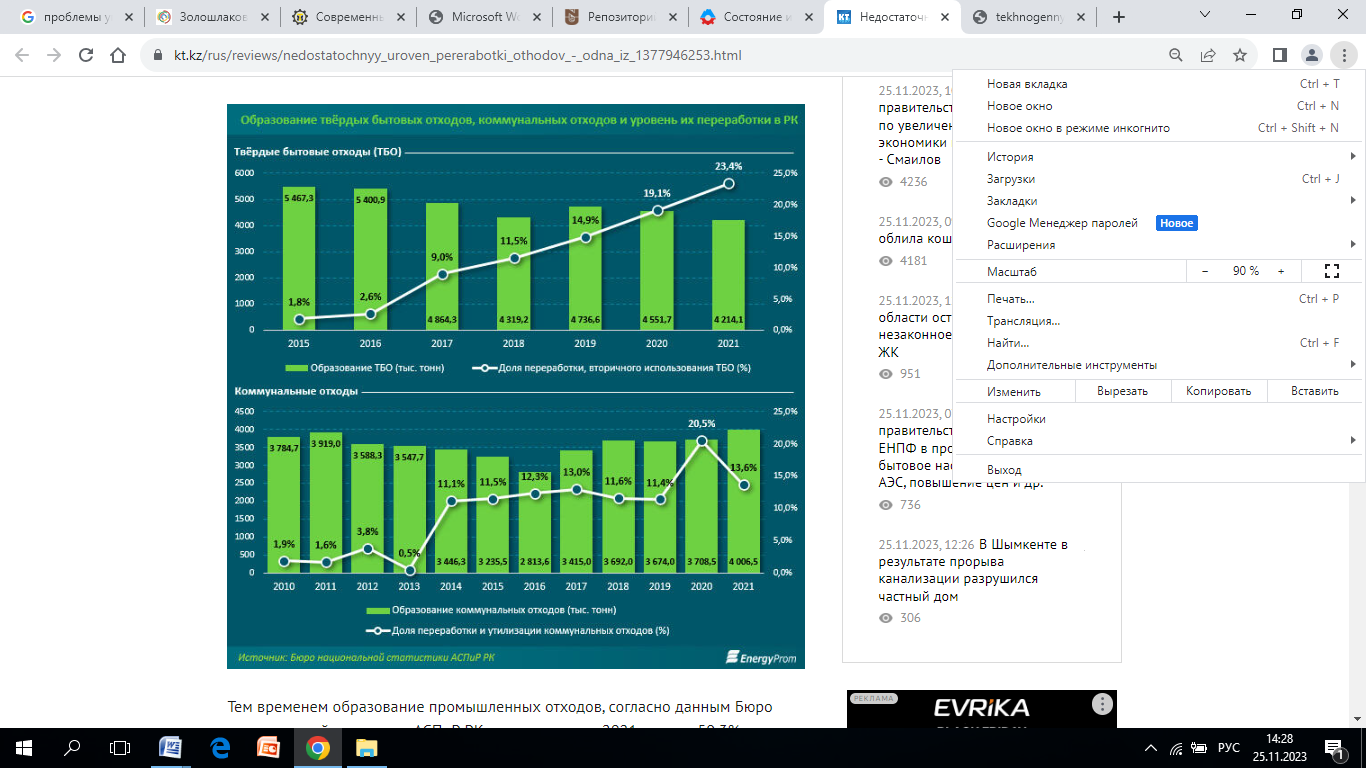
\includegraphics[width=0.6\textwidth]{media/chem2/image66}
	\caption*{Рис.1 - Образование ТБО, коммунальных отходов и уровень их переработки в Казахстане}
\end{figure}

\begin{multicols}{2}
В 2020 году председатель правления Международного центра «зеленых»
технологий и инвестиционных проектов (IGTIPC) Рамазан Жампиисов
прокомментировал следующее: «Проблема обращения с бытовыми отходами
актуальна для Казахстана и требует планомерного решения на основе
использования передового международного опыта. Сортировка и переработка
ТБО в стране на сегодняшний день не превышает 15\%, тогда как в мировой
практике данный показатель равен 70\%»; «Если не заняться проблемой
утилизации бытовых отходов прямо сейчас, уже через несколько лет она
приведет экологию Казахстана к неотвратимым последствиям» {[}14{]}.~

Согласно данным Бюро национальной статистики АСПиР РК образование ТБО,
коммунальных отходов и уровень их переработки в Казахстане представлены
на рисунке 1.

В России в данный момент порядка 90\% отходов отправляется на полигоны и
свалки, и лишь 7\% - на переработку, в то время как в США сжигается лишь
13\% мусора (34\% перерабатывается), в Италии - 19\%, в Германии - 32\%
(48\% получает «вторую жизнь») {[}15{]}.

Сжигание мусора считается общепризнанной технологией его утилизации, так
как она приводит к существенному уменьшению его объемов, а,
следовательно, и к сокращению необходимых для захоронения площадей
полигонов) {[}16{]}. Однако, общепринятое в прошлом веке бесконтрольное
сжигание мусора в печах стало негативным опытом как в Европе, так и в
Америке. Построенные в те годы мусоросжигательные заводы, как оказалось,
загрязняют биосферу в огромном количестве высокотоксичными вредными
веществами, как фураны, диоксины, фосген, синильная кислота и др., а
также зола и шлаки неизвестного состава и с непредсказуемыми свойствами.
Особенно велика при сжигании диоксиновая опасность {[}17{]}. Данные
вещества затем выпадают с осадками, накапливаются в земле и в конечном
итоге оказываются в пищевой цепочке человека, вызывая у него различные
виды канцерогенных заболеваний. По этой причине прямое (без
высокотемпературного воздействия и очистки отходящих газов) сжигание
было запрещено Всемирной организацией здравоохранения (ВОЗ).

В Таблице 1 представлена статистическая информация о применении трех
основных методов утилизации отходов в различных странах: сжигание,
захоронение, компостирование. Сжигание, как метод утилизации отходов, в
большей степени используется в Японии (70\%) и Австрии (73\%), в меньшей
степени (менее 37\%) в других странах. Наименее востребованным данный
способ утилизации является в Англии (7\%) и России (6\%). В Казахстане и
вовсе не используют данный метод.
\end{multicols}

\tcap{Таблица 1 - Процентное соотношение методов утилизации ТБО в различныхстранах}
\begin{longtblr}[
  label = none,
  entry = none,
]{
  width = \linewidth,
  colspec = {Q[152]Q[60]Q[71]Q[87]Q[90]Q[79]Q[73]Q[94]Q[67]Q[73]Q[77]},
  rows = {font = \scriptsize},
  cells = {c},
  hlines,
  vlines,
}
Методутилизации & США & Англия & Франция & Германия & Австрия & Италия & Казахстан & Россия & Япония & {
			Южная
			\\
			Корея
		}\\
Сжигание & 17 & 7 & 37 & 21 & 73 & 13 & - & 6 & 70 & 18\\
Захоронение & 81 & 92 & 53 & 73 & 19 & 84 & 95 & 94 & 17 & 79\\
Компостирование & - & 1 & 10 & 6 & 7 & 3 & - & - & 1 & 2\\
Прочие & 2 & - & - & - & 1 & - & 5 & - & 12 & 1
\end{longtblr}

\begin{multicols}{2}
Распространенный способ утилизации отходов в мире - захоронение отходов
на полигонах. Как видно по таблице, все страны кроме Японии и Австрии
применяют способ захоронения как основной метод утилизации отходов.
Более 70\% ТБО эти страны направляют на захоронение. В системе
захоронения отходов в полигонах предусмотрены разделение отходов на
опасные, бытовые и инертные, также обработка отходов для обезвреживания.
Однако, несмотря на дорогостоящие и многоступенчатые системы фильтрации
отходящих газов, все-таки в окружающую среду проникают загрязнители -
высокотоксичные органические соединения (окислы азота и серы, фенолы,
фураны, полихлорированные дибензо-n-диоксины и дибензофураны и др.).

В странах с развитой экономикой, закон ограничивает содержание в 1
м\textsuperscript{3} выделяемого в окружающею среду газа. Содержание
диоксида азота не должно превышать 0,1·10\textsuperscript{-9}г, а также
дибензофуранов и диоксинов. Такие ограничения диктуют необходимость в
поисках и внедрении современных технологических возможностей утилизации
ТБО с минимальными отрицательными воздействиями на атмосферу.

Технологические и научные достижения позволяют преобразовывать
неутилизируемые ТБО в различные энергоносители - электроэнергию, тепло,
биотопливо и биогаз {[}18{]}. Компостирование {[}19{]} и захоронение
{[}20{]} являются традиционными технологиями обработки отходов, тогда
как технологии анаэробного сбраживания {[}21{]}, сжигания {[}22{]},
пиролиза {[}23{]}, газификации {[}24{]} и гидротермальной переработки
{[}25{]} более эффективны для превращения ТБО в ценные химические
продукты и топливо с добавленной стоимостью. Однако реализация данных
технологий сопряжена определенными трудностями. В частности, важную роль
играет технологическая готовность использования каждого метода {[}26{]}.

Переработка отходов должна быть эффективной, безопасной, а главное
должна быть экологически чистой. Сокращение объемов отходов, повторное
использование, переработка, сортировка, разделение, переработка и
утилизация - это основные этапы комплексного управления отходами
{[}27,28{]}.

Чтобы преодолеть серьезные последствия и риски для здоровья человека в
последнее время было внедрено много новых технологий утилизации отходов.
Пока выбор и применение технологии зависит от разных факторов, включая
экономическое состояние страны, приоритеты и виды образующихся отходов
{[}29{]}. Такие развитые страны как Италия, Япония, США и Великобритания
практикуют концепцию безотходного муниципального управления отходами.
Они внедряют современные способы сбора и хранения отходов, методы
эффективного сжигания,пиролиз, плазменную газификацию, аэробную и
анаэробную очистку {[}30,31{]}. Кроме предварительной обработки и
технологий утилизации отходов, они строго реализуют концепцию 3R
(reduce, reuse andrecycle) сокращение, повторное использование и
переработка {[}32{]}. Развивающиеся страны отстают в гонке новейших
технологий, но у них есть возможности учиться на опыте развитых стран.

С каждым годом растет ценность ТБО как комплексного сырья. Поэтому их
следует подвергать глубокой переработке. Так, итальянская фирма Sorain
Cecchini из 1800 тонн мусора выделяет 55 тонн черных металлов,
производит 25 тонн бумажных волокон, что означает в годовом исчислении
спасение от вырубки почти полмиллиона деревьев. Также из пищевых отходов
делают гранулированное органическое удобрение, из пластика - полимерную
пленку. В целом 55 \% ТБО превращают в товарную продукцию и только
оставшуюся часть сжигают. Полученный при этом шлак также целесообразно
применять для строительных бетонов, покрытия дорог и дренажных засыпок.
Та же итальянская фирма Colari Group имеет 25 дочерних компаний и
является крупнейшим мусоропереработчиком не тольков ЕС, но и в мире.
Так, в ЕС ей принадлежит две трети от всего рынка переработки мусора. В
Японии эта фирма ведет переработку мусора, во Франции - переработку
мусора, выработку удобренийи побочного биогаза (80 \% идет на продажу и
20 \% на собственные нужды). Ежегодно фирма зарабатывает более 1 млрд
евро.

Кроме ТБО глобальную экологическую проблему создает накопление таких
отходов, как промышленные (нефтешлам, металлургические отходы и др.),
сельскохозяйственные, углеотходы (угольная пыль, золошлак). Рассмотрим
более подробно такие распространенные отходы как угольная мелочь (пыль),
золошлак, нефтешлам.

Проблема переработки угольной мелочи существует ввиду того, что
некоторое количество угля (2-4\%) извлекается на поверхность в виде
угольной мелочи, которая не пользуется спросом у потребителей вследствие
низкой калорийности, и вынужденно скапливается в отвалах угледобывающих
предприятий. Это приводит к существенному сокращению земельных площадей
и представляет экологическую угрозу окружающей среде. Поэтому разработка
технологии, позволяющей осуществить переработку угольной мелочи в
полезный продукт, удовлетворяющий по качествам конечного потребителя,
даст решение проблемы как в экономическом, так в экологическом плане.

Также одним из основных источников загрязнения окружающей среды от
углепереработки являются золошлаковые отходы (образующиеся от сжигания
угля в ТЭЦ, котельных и др.). В настоящее время в Казахстане накопилось
500 млн. тонн золошлаковых отходов (ЗШО) и этот объем растет на 19 млн.
тонн ежегодно. При этом, золошлакоотвалы занимают большие площади, а их
строительство требует значительных капитальных затрат со стороны
энергостанций, которые в конечном счете влияют на повышение
себестоимости производства энергоносителей (по данным Казахстанской
электроэнергетической ассоциации). Из ЗШО в Казахстане перерабатывается
около 8 \% золы (менее 1,9 млн тонн). Если использование ЗШМ останется
на этом уровне, тообъём накопленных отходов к 2030 году превысит 1 млрд
тонн. {[}33{]}. Текущая глобальная годовая добыча ЗШО в мире составляет
приблизительно 750 миллионов тонн и в ближайшем будущем, как ожидается,
это количество отходов будет расти.~Данный факт является одним из
серьезных экологических проблем, связанным с угрозой здоровью населения
и экологической безопасности окружающей среды (ущерб для почвы,
растений, атмосферы).~В связи с этим, возникает необходимая потребность
в утилизации и переработки ЗШО. В этом контексте глобальная переработка
ЗШО не только способствует улучшению экологического состояния окружающей
среды, которое является приоритетной задачей, но и дополнительно (кроме
получения энергии) позволит существенно повысить эффективность
переработки угля с получением продуктов повышенной добавочной стоимости
(микросфера, углерод, редкие и редкоземельные металлы, кремний,
алюминий, железо, строительные материалы и др.).

Из данных, представленных на рисунке 2 видно, что наиболее передовыми в
отношении переработки ЗШО являются такие промышленно развитые страны как
Германия, Япония, ЕС, Китай. Как видно, лидирующие позиции по
переработке ЗШО занимают Германия, Япония, ЕС, Китай.
\end{multicols}

\begin{figure}[H]
	\centering
	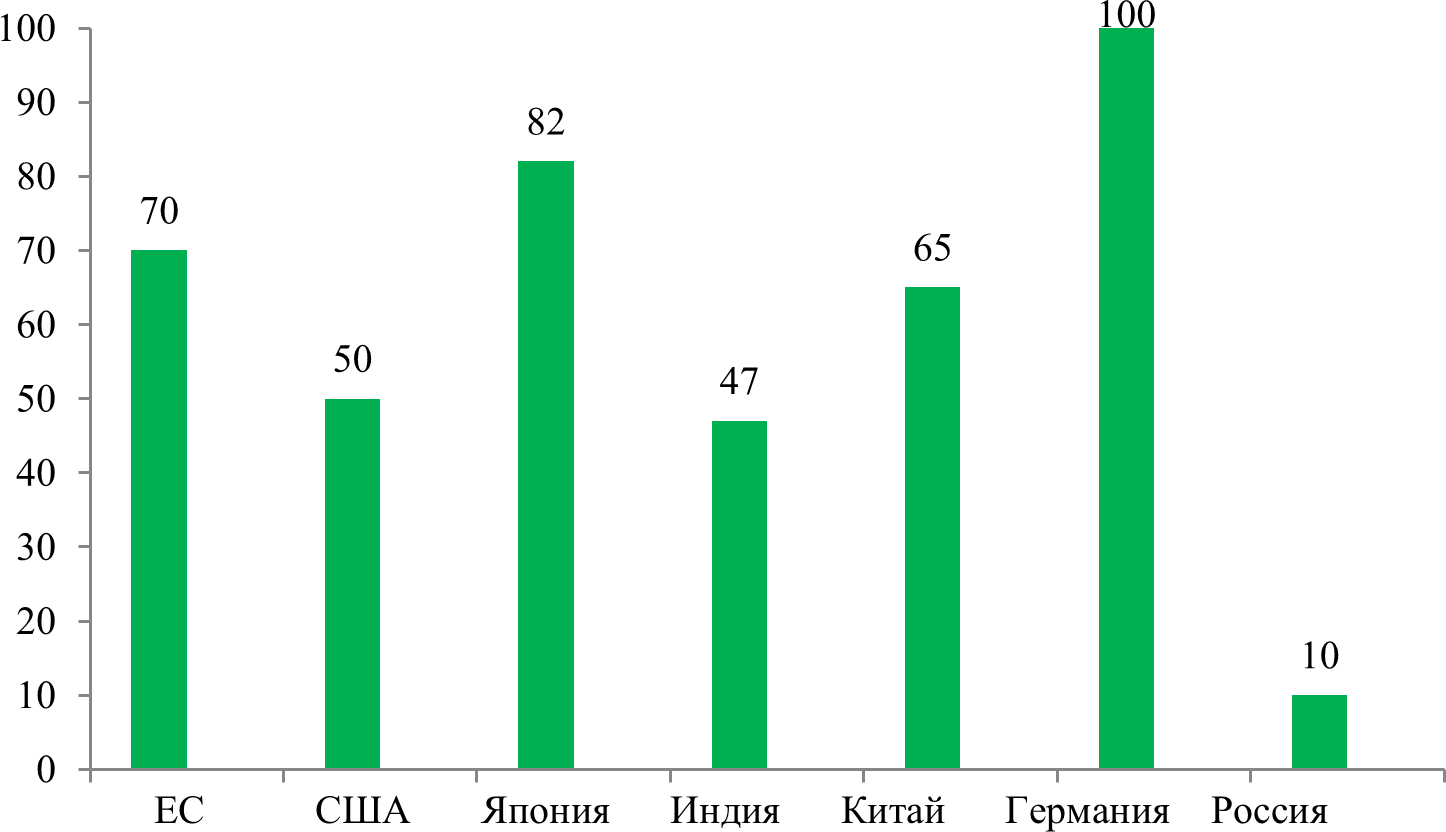
\includegraphics[width=0.6\textwidth]{media/chem4/image10}
	\caption*{Рис.2 - Реализация ЗШО в промышленно развитых странах мира в \% от образования}
\end{figure}

\begin{multicols}{2}
В результате деятельности нефтедобывающих предприятий регулярно
образуются отходы со значительным содержанием нефти: нефтяные шламы
инефтезагрязненные грунты. Это отходы 3-2-го классов опасности в твердом
или пластичном состоянии, требующие специальных методов обращения.
Приэтом темпы образования отходов данного вида заметно превышают темпы
их утилизации. Это свидетельствует о необходимости создания эффективных,
экономичных и экологически чистых технологийпереработки нефтесодержащих
отходов.

Структура нефтешламов представляет собой физико-химическую систему,
включающую в себя нефтепродукты, воду и минеральные добавки (глина,
песок, окислы металлов и т.д.).

На одну тонну перерабатываемой нефти приходится 7 кг нефтешламов, что
приводит к большому скоплению последних в земляных амбарах
нефтеперерабатывающих предприятий. Шламы представляют собой тяжелые
нефтяные остатки, содержащие в среднем 10-56\% нефтепродуктов, 30-85\%
воды, 1,3-46\% твердых примесей. Нефтяные шламы можно использовать по
нескольким направлениям: возврат в производство (при обезвоживании и
сушки) с целью последующей переработки в целевые продукты; использование
их в качестве топлива, однако это связано с большими материальными
затратами. К нефтяным шламам можно добавлять негашеную известь (5-50\%)
и после сушки в естественных условиях использовать в качестве
наполнителя при изготовлении строительных материалов.

{\bfseries Существующие технологии и технологические схемы переработки и
утилизации отходов}

\emph{{\bfseries Общий обзор технологий переработки и утилизации отходов}}

Обзоры предыдущих достижений, включая эволюцию сжигания отходов
(Makarichi и др., 2018 г.) {[}34{]}, анализ общественного мнения (Yuan и
др., 2019 г.) {[}35{]} и анализ государственно-частного партнерства в
области сжигания отходов (Cui и др., 2020) {[}36{]} показали, что
развитие технологии утилизации отходов за последнее десятилетие не
подвергалось должному систематическому анализу. Это особенно актуально в
контексте парадигмы экономики замкнутого цикла.

С целью решения экологическим проблем и вторичного эффективного
использования отходов, в настоящее время по всему миру развитые страны
более широко применяют технологии W2E (Chenetal., 2020) {[}37{]},
представляющие собой процесс получения энергии (в виде электричества
и/или тепла) из отходов. По этой причине W2E (wastetoenergy -- энергия
из отходов) представляет собой реальный потенциал для одновременного
решения проблем отходов и энергии в глобальном масштабе (Skaggsetal.,
2018) {[}38{]}. Это можно объяснить тем, что трансформация и
преобразование отходов в полезную энергию может не только уменьшить
выброс загрязняющих веществ в окружающую среду, но и разнообразить
предоставляемые источники энергии в зависимости от технологических
особенностей каждой страны, региона и местности.
\end{multicols}

\begin{figure}[H]
	\centering
	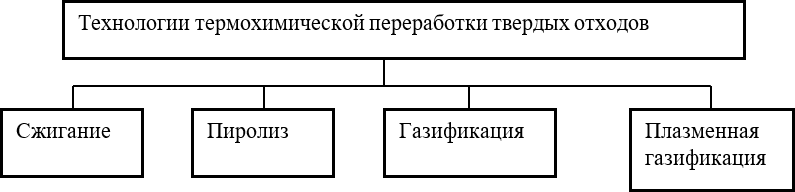
\includegraphics[width=0.7\textwidth]{media/chem4/image12}
	\caption*{Рис.3 - Основные виды переработки твердых отходов}
\end{figure}

\begin{multicols}{2}
Переработкой отходов занимаются более 2500 заводов по всему миру,
используя разные технологии. Метод сжигания мусора в колосниковой печи
используют на 2440 заводах, остальные производства используют метод
пиролиза. Данный метод эффективен в повышении теплотворной способности и
снабжению теплом и электричеством населения. Поэтому превращение отходов
в энергию или другие полезные продукты несет в себе стратегический
синергетический потенциал для сведения к минимуму -- загрязнения,
использование ископаемой энергии и истощение природных ресурсов (Amen
etal., 2021) {[}39{]}.

На рисунке 3 приведены основные виды переработки твердых отходов.

Принцип действия вышеуказанных методов заключается в том, чтобы нагреть
отходы до высокой тем­пературы, при этом возникает разрыв цепей
углеводо­родов на составные части. В основе методов термической обработки
находятся четыре основные стадии: воздей­ствие на отходы высокими
температура­ми, многоступенчатая очистка полученной парогазовойсмеси,
отвод образовавшегося тепла и аккумулирование с дальнейшим применением
образованных ценных мине­ральных и органических продуктов {[}40,41{]}.

\emph{Сжиганием} называется контролируемый процесс окисления отходов
углеводородов, чтобы уменьшить их объем. В процессе сжигания получаются
различные газо­образные продукты: диоксид углерода, моноксид углеро­да
закись азота и прочие газообразные продукты. Также образуются различные
оксиды, а хлор восстановляется до HCl {[}42{]}. Также после сжигания
возникают разные твердые вещества в виде различных металлов, шлака,
стекла и т.д., которые требуют дальнейшего утилизации
или\textbackslash и захо­ронения на полигонах. Сжиганием пользуются в
случаях, когда переработка углеводородных отходов является
затруднительной и\textbackslash или слишком затратной. В процессе
сжигания осуществляются пять парал­лельных или последовательных этапов:
сушка, газифи­кация, воспламенение, горение и дожигание {[}43{]}.

\emph{Пиролиз} является наиболее эффективной и освоенной в промышленном
масштабе из существующих технологий, представляющий собой контролируемое
термическое разло­жение (деструкцию) высокомолекулярной составляющей
органических отходов на низкомолекулярную с получе­нием газообразных
(пиролизный газ) и жидких фракций, а также твердого остаткабез доступа
кислорода {[}44{]}. Пиролиз представляет собой общую стадиюмногих
процессов, таких как сжигание, сжижение, карбонизация, газификация,
которые обычно работают в тесных системах в инертной, восстановительной
или окислительной атмосфере при различных давлениях и времени пребывания
{[}45,46{]}.

В настоящее время пиролиз является наиболее перспективным и исследуемым
термическим направлением переработки таких отходов, как нефтешламы
{[}47{]}. В зависимости от температурных режимов выделяют три вида
пиролиза {[}48,49{]}:

1. Низкотемпературный пиролиз (полукоксование). Температура протекания
процесса - 450-550 °С. Выход пиролизного газа при этом минимален, а
выход жидких продуктов и твердого остатка (полукокса) максимальный.

2. Среднетемпературный пиролиз (среднетемпе­ратурное коксование). Реакция
среднетемпературного пиролиза протекает при температуре 600-800 °С. При
этом наблюдается увеличение выхода пиролизного газа по сравнению с
низкотемпературным пиролизом. Одновременно с этим происходит снижение
выхода жид­кой и твердой фракции. Удельная теплота сгорания получаемого
газа имеет более низкие показатели.

3. Высокотемпературный пиролиз (коксование). Температурный диапазон
протекания процесса состав­ляет 900-1050 °С. При высокотемпературном
пиролизе выход газообразной фракции является максимальным. Выход жидкой
и твердой фракции является минималь­ным. Получаемый газ имеет низкую
теплоту сгорания.

Также в зависимости от скорости нагрева различают медленный и быстрый
(высокоскоростной) пиролиз. При медленном пиролизе скорость нагрева
сырья составляет градусы в минуту или час (условно~подобен процессу
доведения воды до состояния закипания). При высокоскоростном пиролизе
скорость нагрева сырья составляет сотни или тысячи градусов в доли или
единицы секунды (условно~подобен процессу попадания капли воды в
раскаленное масло, т.е. можно представить как~«взрывное вскипание»).
После процесса пиролиза уголь превращается в кокс, полукокс, воду, газы
(Н\textsubscript{2}, СО, Н\textsubscript{2}S, CH\textsubscript{4}),
масло и смолу (фенолы, гетероциклические соединения,нафталин, антрацен).
Выход конечных продуктов термического разложения угля зависит от
характеристики угля, подготовки сырья, режима пиролиза, поглощенной
углем влаги и др. Большую роль играют температура, давление, размер
частиц угля, скорость нагрева, время выдержки, тип реактора и т.д.,
которые определяют общее преобразование углерода и перенос летучих
веществ и, следовательно, распределение продукта {[}50{]}.

\emph{Газификацию} применяют для переработки жидких, твердых и
газообразных органических отходов. Технология процесса заключается в
высокотемператур­ном (1000-1500 °C) взаимодействии органической массы
(нефтешлам, уголь, сланцы и др.) с газифицирующими агентами (водяной
пар, кислород, СО\textsubscript{2}). В результате газификации образуется
синтез-газ (генера­торный газ), а также жидкие смо­листые соединения (до
30\% при температуре 600 °C). Процесс газификации включает 4 основных
этапа: нагревание, сушку, сухую перегонку и газифика­цию. Каждый этап
характеризуется различным температурным интервалом. Нагрев происходит
при темпе­ратуре 100-150 °С, сушка -- при 150-200 °С, сухая пере­гонка --
при 250-800 °С и газификация при -- 1000-1500 °С. При газификации
газовая фаза имеет восстановительные свойства. В результате происходит
минимизация выбросов вредных веществ в окружающую среду по сравнению с
сжиганием. Газификацию можно осуществлять в реакторах с плотными слоями
под давлением и в реакторах с псев­доожиженным слоем. Состав и свойство
получаемого газа зависит от состава сырья и вида окислителя {[}48{]}.
Есть различные способы промышленной газификации углей, из которых
наиболее распространенными являются следующие: в стационарном слое - по
методу Lurgi, в кипящем слое -- по методу Winkler, в потоке -- по методу
KoppersTotzek {[}51{]}. Также применяют новые методы газификации:
процесс в шлаковом расплаве, каталитическая газификация,
гидрогазификация, газификация в циклонных и многоступенчатых
газогенераторах.

\emph{Плазменная газификация} является высоко температурной
разновидностью технологии пиролиза (газификации). По этой технологии в
реакционной камере осуществляется пиролизный процесс с образованием при
высоких температурах (от 1300 до 2000°С) пиролизного газа, который
дожигается в реакторе либо в специальной камере дожигания.

В настоящее время для термической переработки ТБОприменяются установки
инсинераторного типа: продукция совместного Российско-шведского
предприятия «Турмалин» (Санкт-Петербург) - ИН-50, ЭЧУТО-150 (Россия,
Экотехсплав), термические утилизаторы компании Эластек, Инк. (США) и
С.Р. (ATI Mueller, Франция). В рамках реализации национального проекта
«Экология» строится несколько мусоросжигающих заводов по технологии
Hitachi (Япония) {[}52{]}.

Переработка угольной мелочи в процессе газификации пылевидного топлива в
потоке является одним из перспективных методов получения горючего газа
из угля {[}53{]}. Основными преимуществами этого метода является высокая
интенсивность процесса, сырьем для которого также могут являться
низкосортные, влажные и зольные топлива, которые содержит много мелочи,
и сжигание таких топлив затруднено в слоевых аппаратах.

Одним из основных способов утилизации нефтяных шламов является сжигание
в печах различной конструкции (камерных, кипящего слоя, барабанных и
др.). Печи кипящего слоя широко используют для отходов, содержащих не
более 20\% твердых примесей. При сжигании шламов, содержащих до 70\%
твердых примесей, распространение получили вращающиеся печи барабанного
типа.

Традиционно собранные в процессе зачистки резервуаров нефтешламы
жидко-вязкой консистенции подвергаются разделению на нефтепродукт, воду
и твердые механические примеси. Эта фаза переработки имеет своей целью
извлечение из шламов нефтепродуктов с исходными свойствами и их
использование по прямому назначению. Существуют два основных способа
фазового разделения жидковязких нефтешламов − механический и химический.
Для более глубокой очистки нефтепродуктов иногда прибегают к комплексной
технологии.

На рисунке 4 приведены основные методы утилизации нефтешлама {[}54{]}.
Как видно, кнефтешламу с содержанием углеводородных загрязнителей в
интервале 6-25 масс.\% целесообразно применить физико-химические методы,
основными из которых являются экстракция нефтяных загрязнителей
растворителем и пиролиз углеводородного остатка после восстановления
(отгонки) растворителя.
\end{multicols}

\begin{figure}[H]
	\centering
	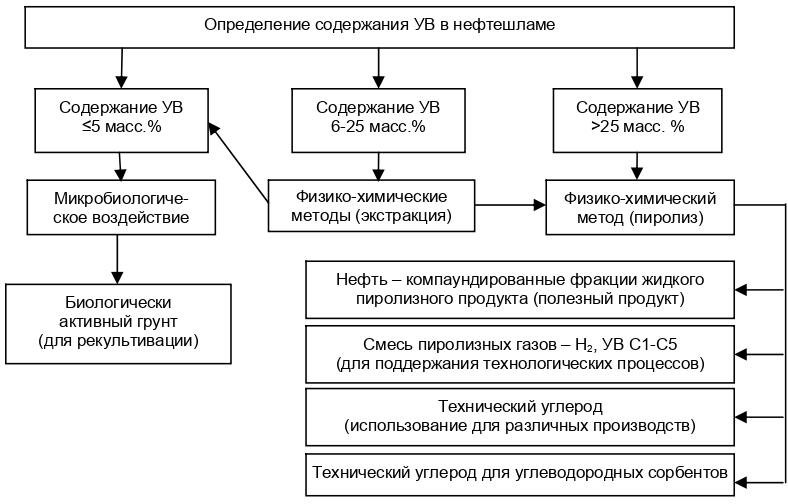
\includegraphics[width=0.8\textwidth]{media/chem2/image67}
	\caption*{Рис.4 − Основные методы утилизации нефтешлама {[}54{]}}
\end{figure}

\begin{multicols}{2}
B {[}19-24{]} представлены основные методы утилизации отходов, среди
которых, как ранее указывалось, можно особо отметить пиролиз. Например,
технология высокоскоростного пиролиза твердого сырья в установках с
твердым теплоносителем основана на методе Галотер, изобретенном в 1947
году инженером И. С. Галынкером и разработанном Энергетическим
институтом ЭНИН (Москва). Сущность способа заключается в том, что
пиролиз сырья происходит при его смешивании с горячей золой во
вращающемся барабане реактора без доступа кислорода. Органическое
вещество разлагается с образованием парогазовой смеси, которая при
охлаждении образует различные фракции синтетических нефти и газа.
Полукокс сжигается в аэрофонтанной топке. Часть горячей золы
возвращается в реактор для нагрева свежей порции сырья, избыток золы
охлаждается и удаляется из процесса. Тепло золы, дымовых газов и
синтез-газа используется в котле-утилизаторе для получения пара с
энергетическими параметрами для производства тепловой и электро энергии.
Технология освоена на коммерческом и промышленном уровнях.

\emph{{\bfseries 3.2 Технология сжигания отходов}}

Сжигание является наиболее применяемым методом утилизации отходов.
Конечные продукты прямого сжигания -- зола и значительные объемы
токсичных летучих вещества (бензапирена) и хлорсодержащих (диоксинов),
выбрасываются в окружающую среду. С учетом этого эффективная
(экологически чистая) утилизация должна строиться не на простом
сжигании, а на глубокой переработке с промежуточной нейтрализацией этих
компонентов.

В странах «Большой семерки» наибольшее распро­странение для сжигания
отходов получили печи с кипя­щим слоем. Так, например, в США была
разработана и представлена установка, предназначенная для сжигания
жидких углеводородных отходов. Установка обладает производительностью в
4 м\textsuperscript{3}/ч. Температура сжигания составля­ет 1000-1200 °C.
В Германии сжигание углеводородных отходов производят в вертикальных
печах с кипящим слоем. Температура сжигания составляет до 800 °C.
Образующиеся при этом дымовые газы с температурой около 900 °C
охлаждаются и поступают обратно в цикл. С целью сжигания нефтесодержащих
осадков из очистных сооружений рентабельнее использовать бара­банные
печи.

Помимо печей различной конструкции, распростра­нение на территории России
получила установка для сжигания жидких нефтесодержащих отхо­дов типа
«Форсаж-1» или «Вихрь». Производительность установок составляет до 50
кг/ч для «Форсаж--1» и до 10 т/ч для «Вихрь--1» соответственно.
Температура сжигания - 1000±100 °C. Содержание минеральных примесей и
влаги не должно превышать 80\%.

Принципиальная технологическая схема технологии сжигания {[}55{]}
представлена на рисунке 5. Данная технология осуществляется в режиме
высоких температур, что позволяет уничтожить вредные продукты горения и
создать большое количество тепла, способное нагреть пар, который
используется в дальнейшем при работе турбогенератора. При такой
переработке выделенные для переработки отходы производства и потребления
превращаются в возобновляемые источники энергии.
\end{multicols}

\begin{figure}[H]
	\centering
	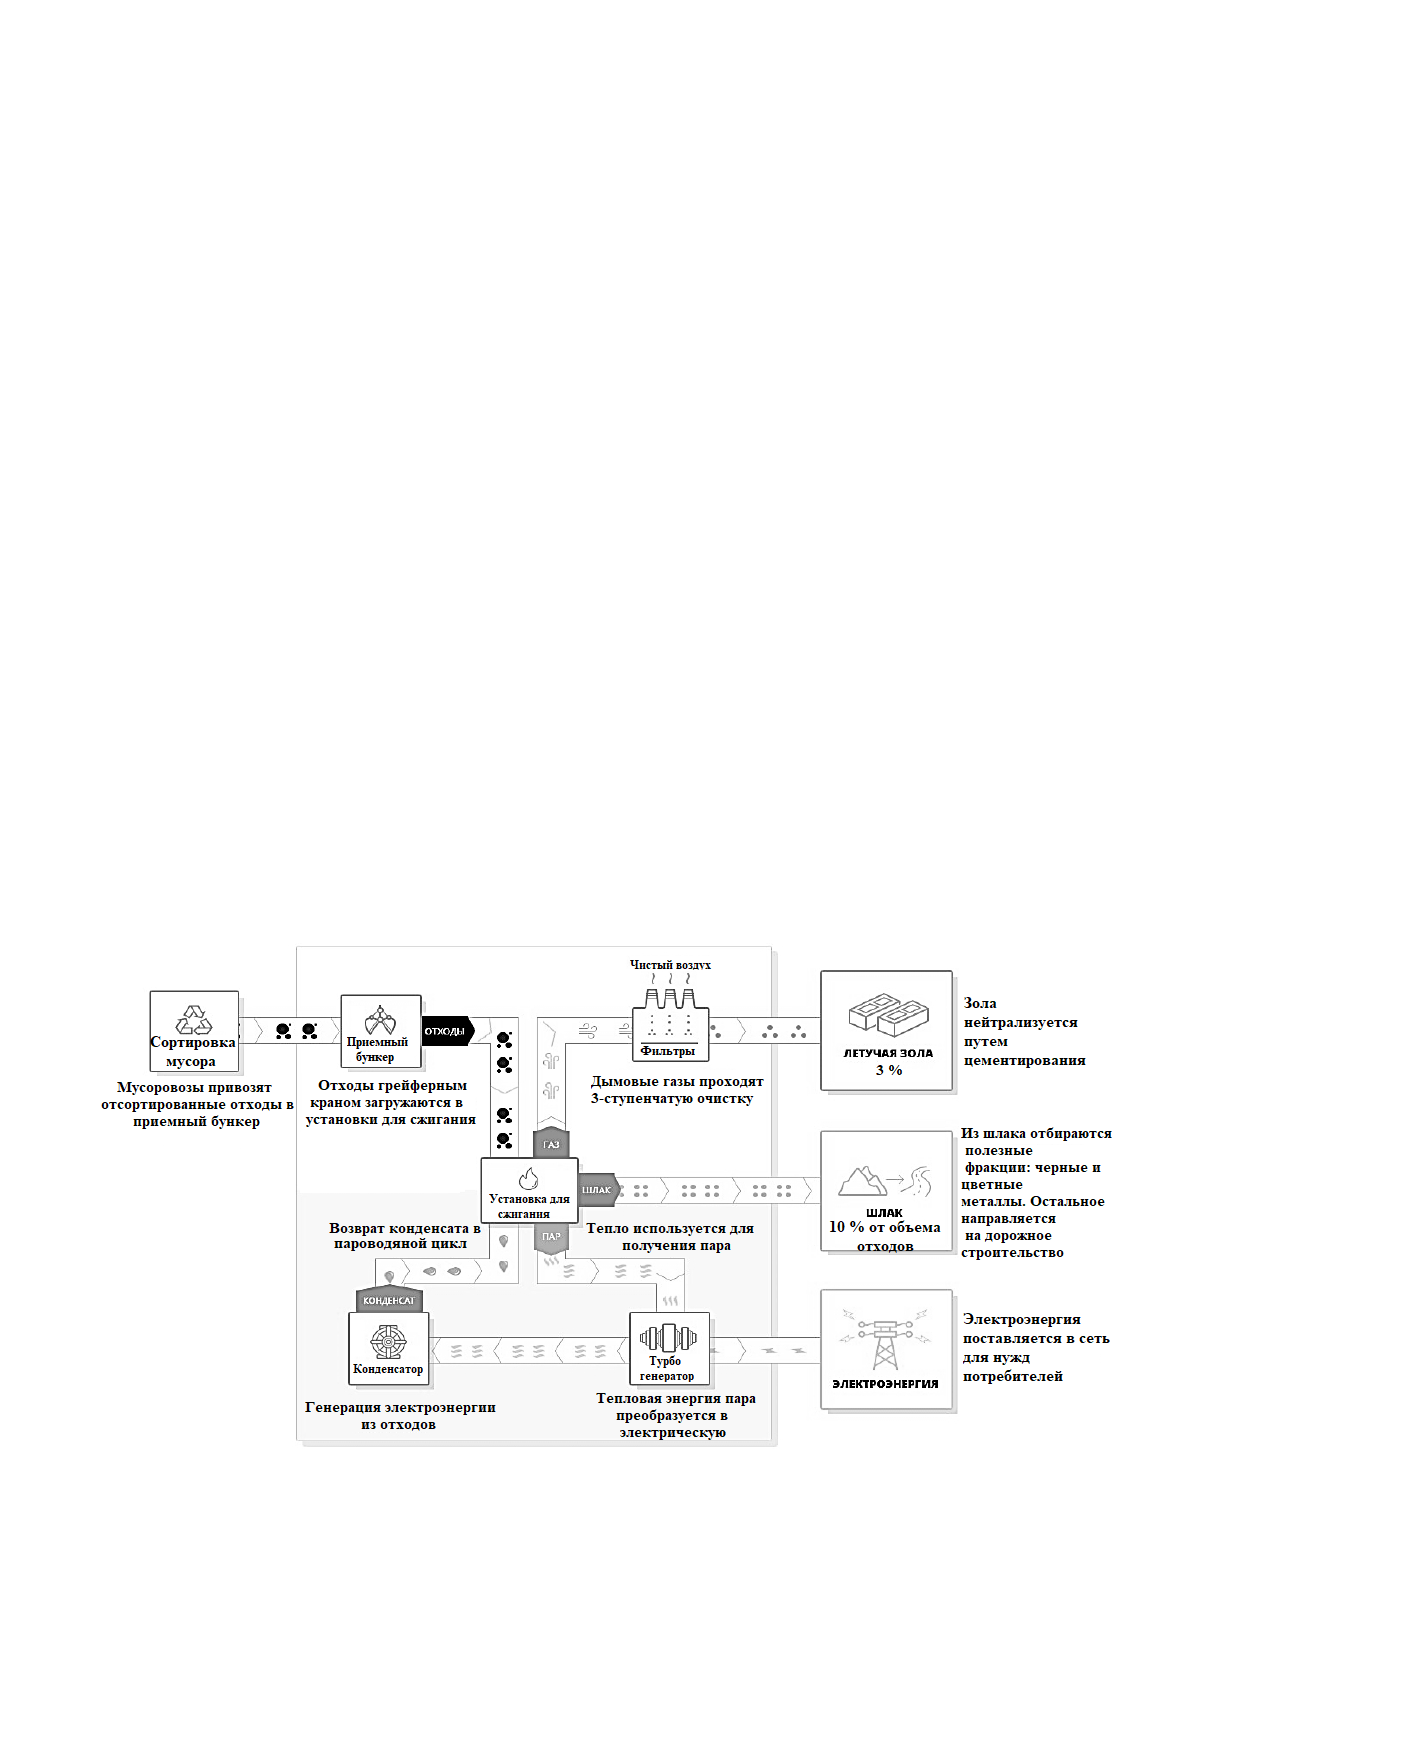
\includegraphics[width=0.8\textwidth]{media/chem2/image68}
	\caption*{Рис.5 - Принципиальная технологическая схема технологии сжигания {[}55{]}}
\end{figure}

\begin{multicols}{2}
В результате целого ряда технических операций (рисунок 5) переработанные
отходы поступают в установку для сжигания. В технологии энергия дымовых
газов преобразуется в котле в энергию пара, который затем используется
для производства электроэнергии. Пар, поступающий на производство
энергии, и дымовые газы циркулируют в разных контурах и никогда не
смешиваются в технологическом процессе.

Замкнутость производственного цикла обеспечивается поступлением пара с
турбины по трубам в производство конденсата, который преобразуется
обратно в воду и возвращается в котел. Эффективность технологического
цикла подтверждается тем, что после процесса сжигания объем оставшихся
отходов составляет около 10\% от общего объема.

Как ранее отмечалось, в результате переработки отходов наряду с энергией
получаются сопутствующие продукты переработки, в том числе шлак. Шлак,
который образуется в котле, составляет 30\% от массы и 10\% от входящего
объема отходов иимеет такой же класс опасности, как и несортированные
отходы. Шлак направляют на охлаждение, а затем выгружается на ленточный
транспортер. В процессе работы из шлака отбирают черные и цветные
металлы, которые впоследствии направляют на следующий этап переработки
{[}56{]}. Данная технология представляет собой многостадийный процесс с
достаточно простым оборудованием, которое может быть особо актуальным в
период перехода экономики в стадию импортозамещения.

На рисунке 6 приведена схема установки для сжигания отходов
мусороперерабатывающего завода {[}57{]}. Твердые отходы поступают в
мусоросборник, а затем погружным ковшом передаются в печь для сжигания.
Образовавшиеся дымовые газы проходят через систему охлаждения и очистки,
после чего выбрасываются в атмосферу. При этом, многоступенчатая сухая
очистка дымовых газов обеспечивает выполнение экологических стандартов
производственной деятельности. Шлаки охлаждают и транспортиром после
отделения металлических материалов с помощью электромагнитного
сепаратора направляют в сборник.
\end{multicols}

\begin{figure}[H]
	\centering
	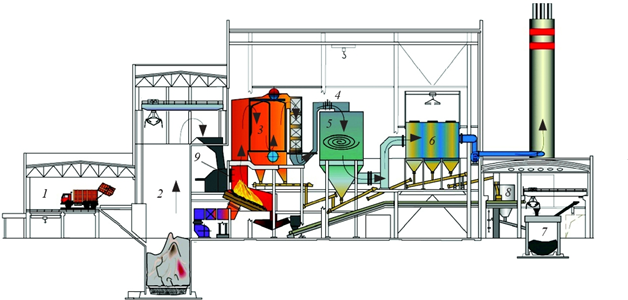
\includegraphics[width=0.8\textwidth]{media/chem2/image69}
	\caption*{Рис. 6 - Схема установки для сжигания твердых отходов {[}57{]}}
	\caption*{\normalfont\emph{1 - приемное отделение; 2 - приемный бункер отходов; 3 -
котлоагрегатор; 4-6 - отделение газоочистки;7, 8 - шлаковое отделение; 9
- загрузка ТКО в печь}}
\end{figure}
\begin{figure}[H]
	\centering
	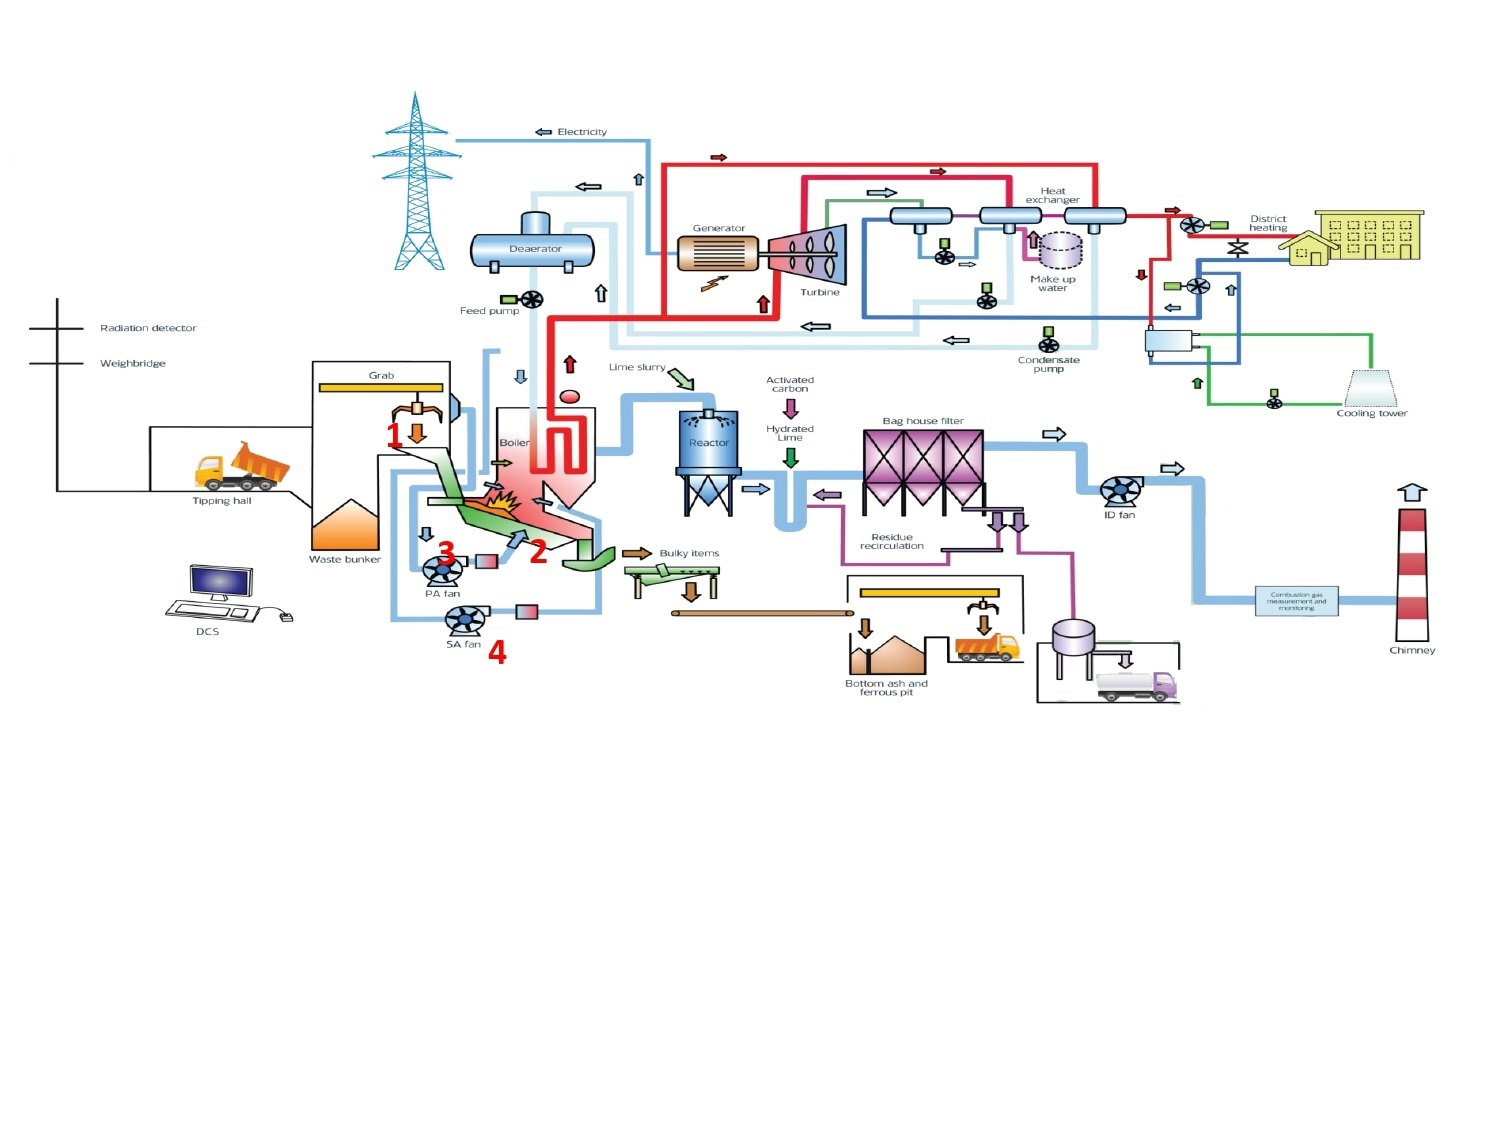
\includegraphics[width=0.8\textwidth]{media/chem2/image70}
	\caption*{Рис.7 - Технологическая схема сжигания}
\end{figure}

\begin{multicols}{2}
В качестве примера успешного проекта, характеризующего динамику развития
предприятий по термической переработке отходов, следует привести
перерабатывающий завод в Шотландии. Функционирование предприятия по
термической переработке осуществляет компания Octopus Renewables в
промышленной зоне Олдхолл в Эрвине с населением примерно 370 тысяч
человек. Данное предприятие производит 17 МВт электроэнергии, что
позволяет снабжать энергией 30 000 домов, а также обеспечивать теплом и
паром прилегающие к территори и промышленные предприятия {[}58{]}.

На рисунке 7 приведена технологическая схема сжигания, разработанная
компанией CNIM (Франция).
\end{multicols}

\begin{figure}[H]
    \centering
    \begin{subfigure}[t]{0.9\textwidth}
        \centering
        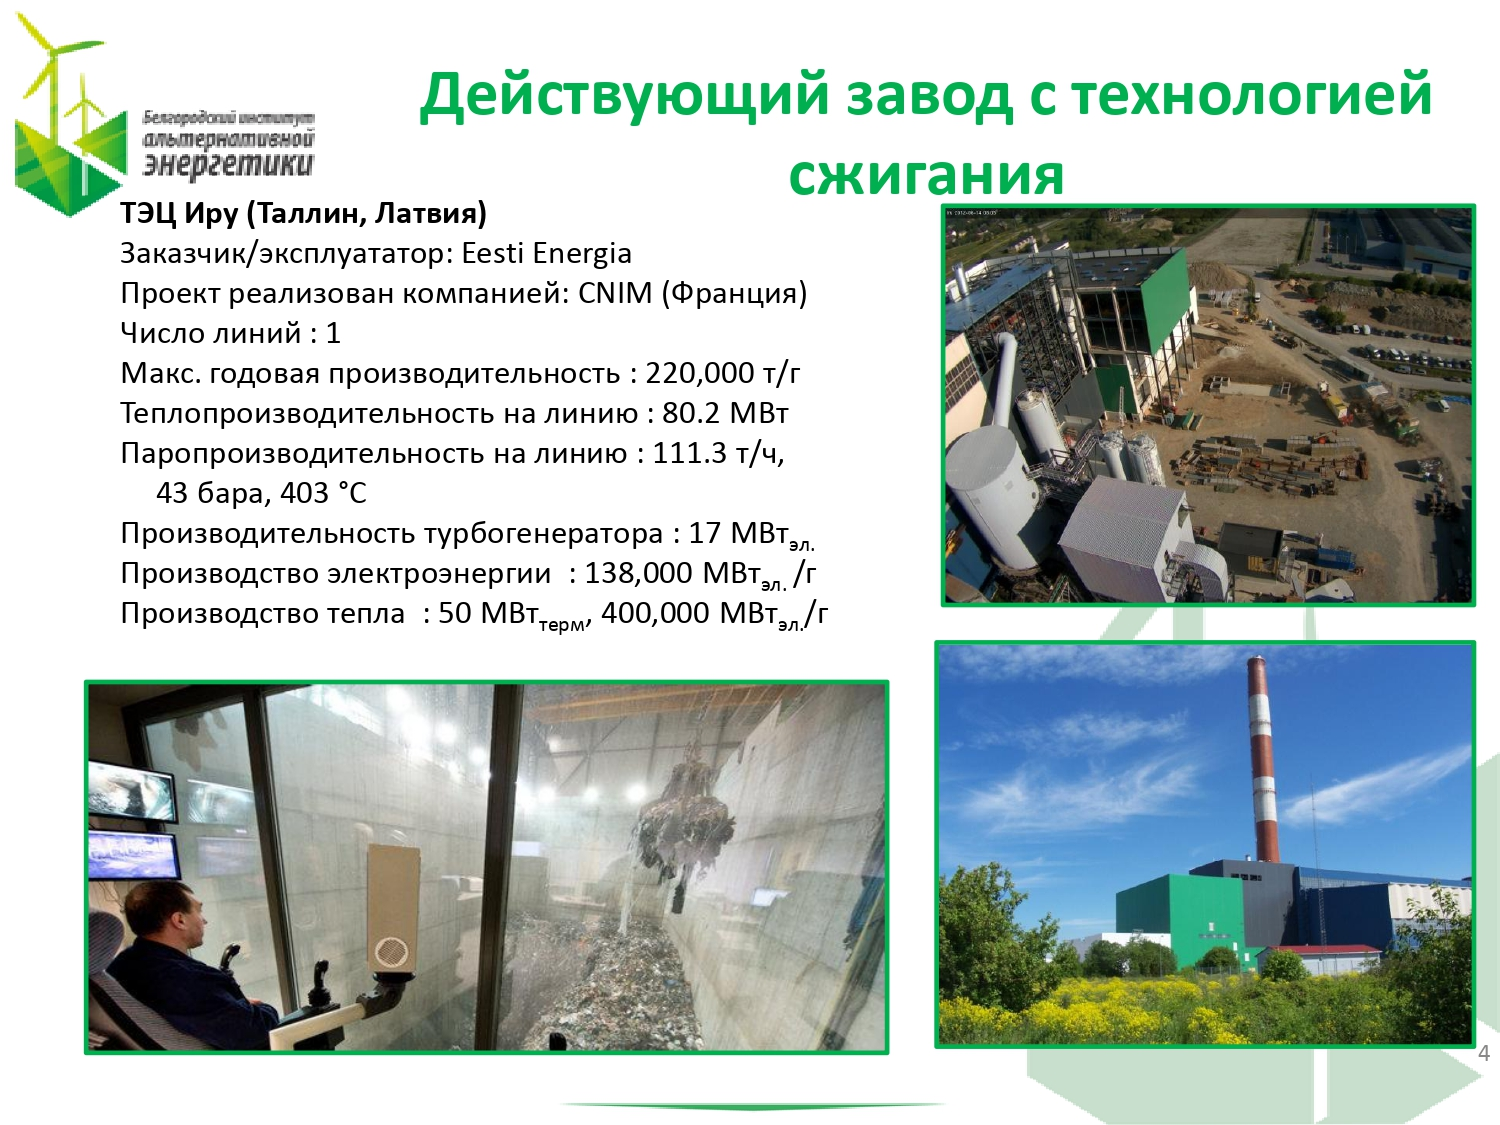
\includegraphics[width=\textwidth]{media/chem2/image71}
    \end{subfigure}
    \begin{subfigure}[t]{0.45\textwidth}
        \centering
        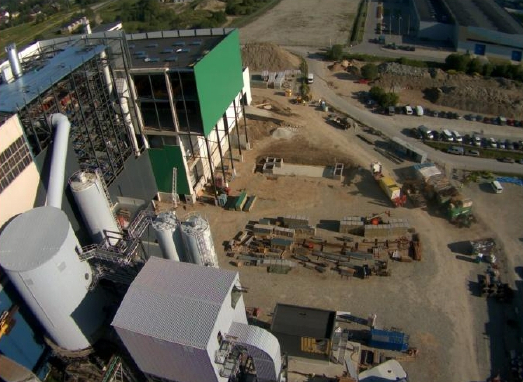
\includegraphics[width=\textwidth, height=6cm]{media/chem2/image71.1}
    \end{subfigure}
    \hspace{-5pt}
    \begin{subfigure}[t]{0.45\textwidth}
        \centering
        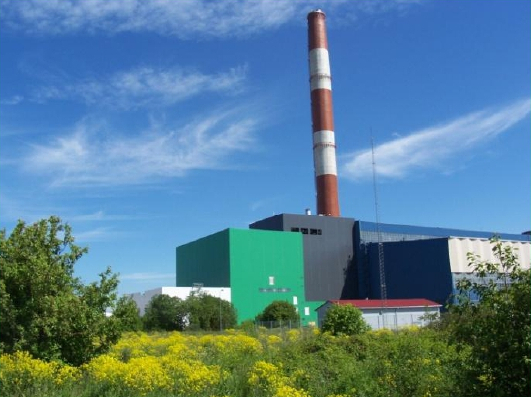
\includegraphics[width=\textwidth, height=6cm]{media/chem2/image71.2}
    \end{subfigure}
    \caption*{{\bfseries Рис.8 - Действующий завод в Таллине (Латвия)}}
\end{figure}

\begin{multicols}{2}
Краны ТБО загружают отходы на топочную решетку через загрузочную воронку
и лоток (1). Автоматически управляемые гидроцилиндры подают отходы на
поверхность обратно-переталкивающей решетки (2), которая является
наиважнейшей частью в сжигании отходов. Она оснащена движущимися
колосниками (2). Решетка имеет наклон 26° относительно горизонтали, от
питателя в сторону выгрузки остаточных продуктов горения. Решетка
состоит из чередующихся подвижных и неподвижных колосников. Подвижные
колосники медленно перемещают отходы на наклонной решетке. Это
обеспечивает их постоянное перемешивание и одинаковую толщину слоя
горящих на решетке отходов. Горящая масса отходов проталкивается
обратно, к началу решетки, при этом все фазы горения, такие каксушка,
воспламенение и горение, происходят одновременно. Вентилятор первичного
воздуха (3) через зазоры решетки обеспечивает воздух для горения слоя
отходов на решетке. Этот вентилятор и вентилятор над пламенем решетки
поставляют вторичный воздух (4), забираемый из приемного отделения, в
зоне приемного бункера, что предотвращает распространение дурных запахов
вне здания. Первичный воздух подогревается при помощи парового
подогревателя воздуха.

Согласно данной технологической схеме в результате сжигания получаются
продукты: электрическая и тепловая энергия, а также шлаки, из которых в
дальнейшем можно извлекать ценные металлы и применять в качестве
строительных материалов.

Компанией CNIM (Франция) реализован проект в Таллине (Латвия).
Заказчик/эксплуататор-- компания Eesti Energia. Это действующий завод с
максимальной годовой производительностю: 220000т/год (рисунок 8).
Числолиний: 1. Теплопроизводительность на линию: 80,2 MВт.
Паропроизводительность на линию: 111,3 т/ч, 43 бара, 403°C.
Производительность турбогенератора: 17 MВт\textsubscript{эл}.
Производство электроэнергии: 138000 МВт\textsubscript{эл.}/год.
Производство тепла: 50 МВт, 400000 МВт/год.

\emph{{\bfseries Технология пиролиза отходов}}

На рисунке 9 приведены различные виды отходов, которые используют для
пиролиза: коммунальные, промышленные, сельскохозяйственные, углеотходы.
\end{multicols}

\begin{figure}[H]
	\centering
	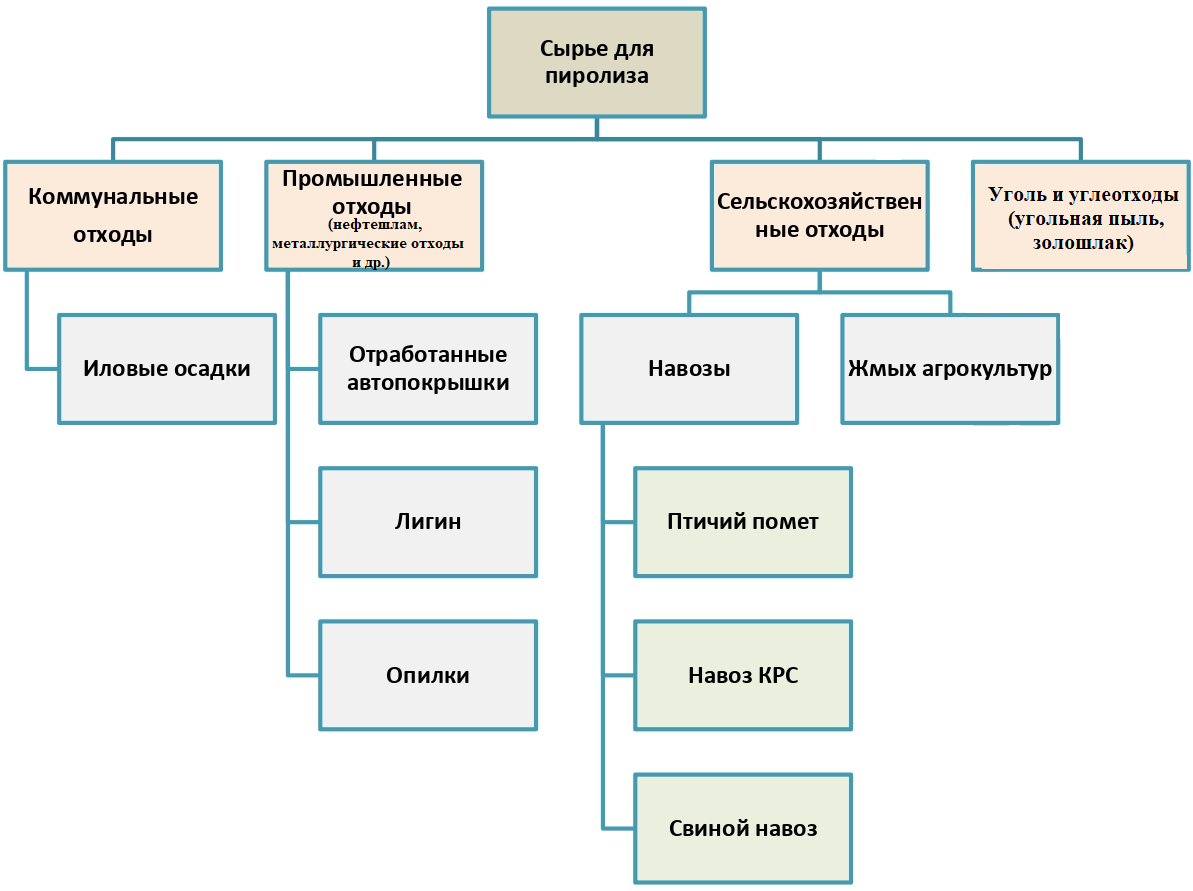
\includegraphics[width=0.9\textwidth]{media/chem2/image72}
	\caption*{Рис.9 - Виды сырья для пиролиза}
\end{figure}

\begin{multicols}{2}
На рисунке 10 приведена технологическая схема пиролиза, в котором
твердые отходы (ТБО, угольная мелочь и др.) предварительно измельчают,
сушат и подают в реактор пиролиза, в результате которого на выходе
получают электрическую и тепловую энергию, а также различные твердые
продукты (в зависимости от исходного сырья).

Пиролизная установка по переработке угля и углеотходов в синтетическое
топливо (рисунок 11) введена в эксплуатацию в 2012 году в г.Брисбэйн,
Австралия. Проект реализован компанией Ener-Core (Австралия). Мощность
установки - 16000 тонн угля в год; производство синтетического топлива -
4128000 литров/год; площадка - 0,4 га.
\end{multicols}

\begin{figure}[H]
	\centering
	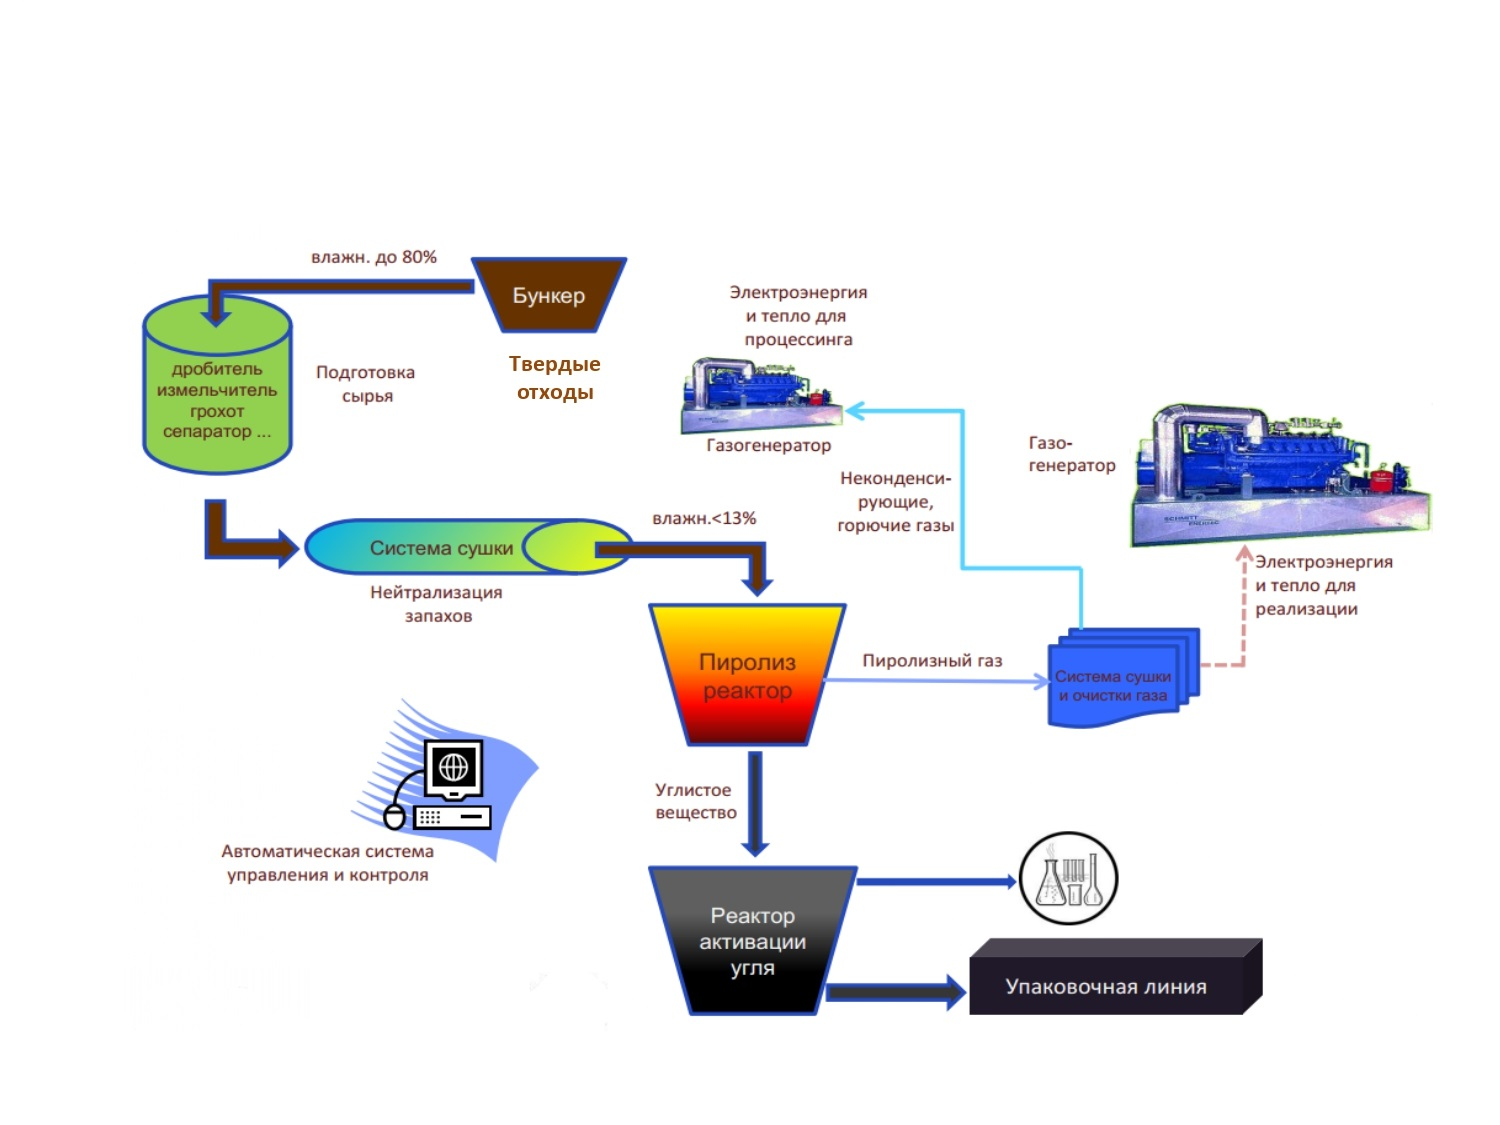
\includegraphics[width=0.8\textwidth]{media/chem2/image73}
	\caption*{Рис.10 - Технологическая схема пиролиза}
\end{figure}

\begin{figure}[H]
	\centering
	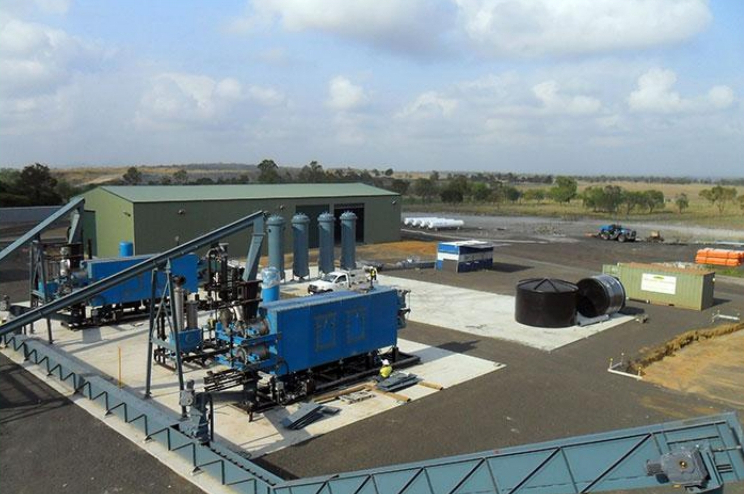
\includegraphics[width=0.6\textwidth]{media/chem2/image74}
	\caption*{Рис.11 - Пиролизная установка по переработке угля в
синтетическое топливо}
\end{figure}

\begin{multicols}{2}
На рисунке 12 показана принципиальная схема разработанной установки
{[}59{]}. Исходное сырьё -- нефтесодержащие отходы (нефтешлам и др.) из
резервуара 1 через распределительное устройство 2 подаются в камеру
пиролиза 3.
\end{multicols}

\begin{figure}[H]
	\centering
	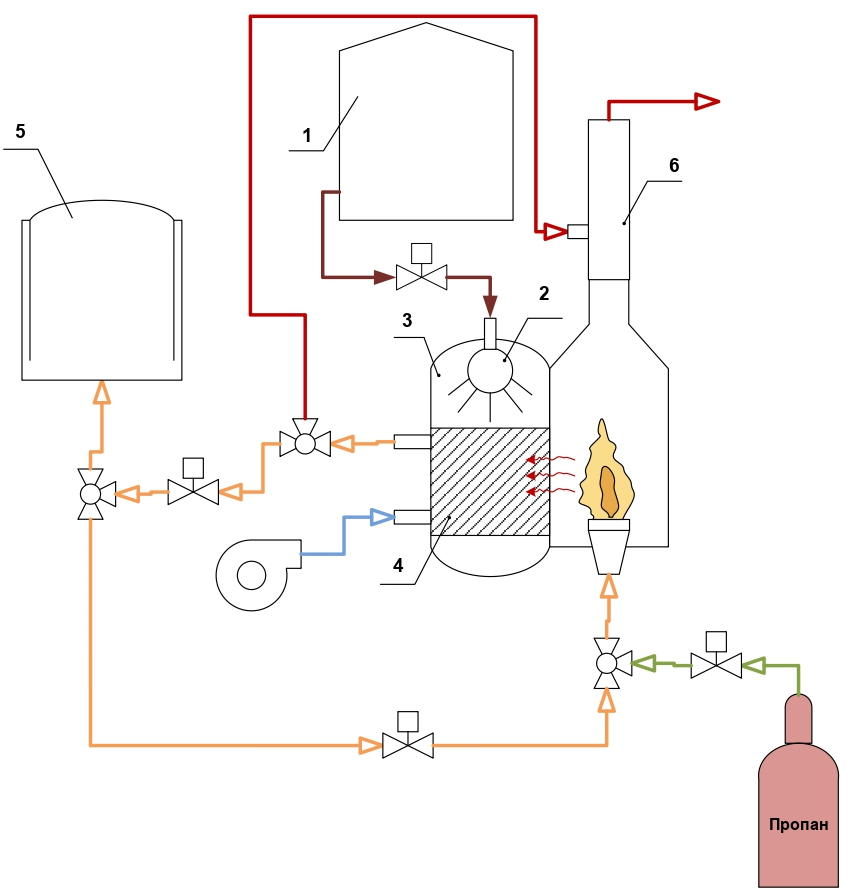
\includegraphics[width=0.5\textwidth]{media/chem2/image75}
	\caption*{Рис.12 - Структурная схема технологической установки
переработки отходов нефтепродуктов методом низкотемпературного пиролиза
{[}59{]}:}
    \caption*{\normalfont\emph{1-резервуар, 2- распределительное устройство, 3-камера пиролиза,4-насадка в виде дисперсного материала,5- газгольдер,6-труба}}
\end{figure}

\begin{multicols}{2}
Нагрев и пиролиз жидкой составляющей, а также поддержание необходимого
уровня температуры осуществляется за счет подвода тепла, выделяющегося
присжигании топливного газа в газовой горелке. Загружаемые через
распределительное устройство 2 в насадку 4 нефтеотходыподвергаются
пиролизу в камере пиролиза 3, образующей реакционный объем. В процессе
нагрева и пиролиза отходов интервале температур 550-600
\textsuperscript{o}C идет интенсивное выделение газа. Образующиеся
газообразные продукты пиролиза направляются в газгольдер 5.

Тепло для процесса пиролиза вырабатывается при помощи газовой горелки,
которая в момент запуска работает на пропане, а затем достигнув нужной
температуры переключается на пиролизный газ. Подогрев газообразной
составляющей пиролизным газом позволяет существенно повысить
энергетические показатели эффективности технологического процесса, т.к.
вводимый предварительно подогретый поток газа не снижает существенно
температуру, что позволяет минимизировать дополнительный подвод тепла за
счет подачи электроэнергии. Высокий уровень температур позволяет
поддерживать высокую эффективность протекания реакций химико-термической
обработки газообразной составляющей. Таким образом, предлагаемая
технологическая установка позволяет эффективно проводить переработку
отходов нефтепродуктов при минимальном воздействии на окружающую среду.

Авторами в работе {[}54{]} разработана технологическая схема утилизации
нефтесодержащих отходов (рисунок 13), включающая отделение углеводородов
растворителем, пиролиз и разделение нефтепродуктов на фракции. Схема
позволяет перерабатывать весь комплекс нефтесодержащих отходов
предприятий нефтедобычи с получением полезной продукции: нефти,
биоактивных грунтов, технического углерода. Применение углеводородного
растворителя позволяет обеспечивать высокую степень очистки твердой фазы
нефтесодержащих отходов от нефти. Содержание нефтепродуктов находится в
интервале 1,2-24,3 г/кг.
\end{multicols}

\begin{figure}[H]
	\centering
	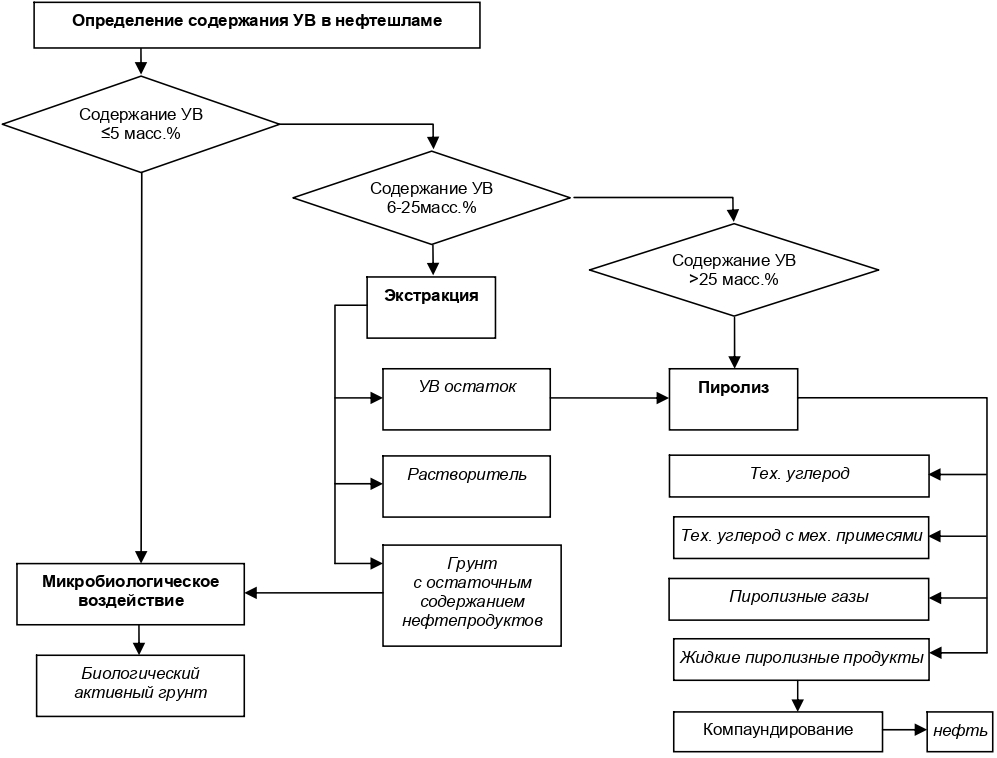
\includegraphics[width=0.8\textwidth]{media/chem2/image76}
	\caption*{Рис.13 - Технологическая схемаутилизации нефтесодержащих
отходов {[}54{]}}
\end{figure}

\begin{multicols}{2}
Для повышения выхода легких фракций углеводородов исследован процесс
быстрого пиролиза при температуре 650 °С. Получаемые продукты пиролиза
представлены н-алканами и изо-алканами. Наибольший вклад в состав вносят
углеводороды с содержаниематомов углерода от С\textsubscript{6} до
С\textsubscript{26}. По данным ГХ-анализа, содержание тяжелых
углеводородов (С\textsubscript{12} и выше) составляет от 46\% до 73\%.
Из продуктов пиролиза возможно выделение более 25\%-60\% бензиновой
фракции. Отмечается существенная доля дизельной фракции. В составе
пиролизных углеводородов содержится большое количество изомерных
алканов, которые обладают высоким октановым и цетановым числами.

Данная технологическая схема реализована в макете установки утилизации
нефтезагрязненных грунтов производительностью 30 л/час по
перерабатываемому отходу.

С целью переработки тяжелых нефтешламов и при­родных битумных
месторождений в легкую нефть был разработан мини-завод
«Потрам--Нефтешламы--Легкая нефть». Данный агрегат позволяет
перерабатывать поряд­ка 50-100 т/сутнефтеотходов. Он включает в себя
следую­щие стадии переработки: низкотемпературный пиролиз, разделение
парогазовой смеси (получение легкой нефти), сепарация и удаление воды
{[}60{]}.

Компанией IPEC была разработана и введена в экс­плуатацию в 2014 году
установка термической деструк­ции (УТД-2) {[}61{]}. Испытание и ввод в
эксплуатацию УТД-2 проводились на Вынгапурском нефтегазовом
месторож­дении в Тюменской области. Среди преимуществ данной установки
отмечают возможность переработки сухих и жидких углеводородных отходов,
а также энергонезави­симость установки.

Еще одной установкой для переработки любых орга­нических продуктов,
включая тяжелые остатки и отходы, образующиеся в результате
нефтепереработки, является пиролизная установка компании ООО НПФ
«Энергия». Сущность работы данной установки основана на тех­нологии
термоудара, т.е. мгновенном нагреве отходов (скорость нагрева
\textasciitilde104 град/сек). Среди преимуществ технологии термоудара
можно выделить первоначально­го объема отходов в несколько раз (в 10 и
более). Однако для поддержания работоспособности данной технологии
требуются высокие энергетические затраты {[}62{]}.

В таблице 2 приведены экономические и технологические показатели
пиролизных установок.
\end{multicols}

\tcap{Таблица 2 - Экономические и технологические показатели пиролизных установок}
\begin{longtblr}[
  label = none,
  entry = none,
]{
  width = \linewidth,
  colspec = {Q[40]Q[108]Q[550]Q[135]Q[100]},
  rows = {font = \small},
  cells = {c},
  hlines,
  vlines,
}
№ & \textbf{Компания,			страна} & \textbf{Сырье} & \textbf{Объем			реактора, поизводительность} & \textbf{Цена,			тыс.долл.}\\
1 & Экострой
			ПВ, ТОО,
			Атырау, Казахстан & Углерод-содержащие
			отходы
			2-5 класса опасности
			(в т.ч. отходы
			резины, отходы
			при добыче нефти и газа; отработанные
			масла;
			шламы
			нефти и нефтепродуктов; отходыЛКМ;
			медицинские
			отходы
			и др.) & 8,5			м\textsuperscript{3} & 54,0\\
2 & Beston
			Group
			Co., Ltd, Китай & Нефтешлам,
			отходы резины, пластик & 1,5-30
			тонн/сутки & 45,0-688,9\\
3 & {
			ПТК
			Пиролиз-Экопром
			ООО,
			\\Россия
		} & {
			Углеродосодержащие
			промышленные
			отходы2-5
			класса опасности,
			в т.ч.~
			\\отходы
			резины, нефтешлам, нефтесодержащие
			отходы, мазут, битумные отходы, каучуки,
			масла, медицинские отходы, загрязненный
			обтирочный материал, тара полиэтиленовая
			загрязненная, пленка загрязненная
			промасленная, железнодорожные
			деревянные шпалы, загрязненные «хвосты»
			ТБО/ТКО и др.).~
		} & 2,6			м\textsuperscript{3} & 41,6\\
4 & Ассоциация
			предприятий БМП, Россия & Нефтешламы,
			промышленные и бытовые углеродосодержащие
			отходы 1-5 класса опасности & {5			м\textsuperscript{3}\\7			м\textsuperscript{3}\\10			м\textsuperscript{3}\\20			м\textsuperscript{3}} & {
			26,2
			\\
			32,3
			\\
			40,9
			\\65,5
		}\\
5 & {
			«ТТ
			ГРУПП»
			ООО,
			\\Россия
		} & Уголь,
			древесина, шины, пластики, отходы
			электроники, нефтешламы, нефтезагрязненные
			грунты, медицинские отходы, отходы
			деревообработки, отходы ЛКМ, отработанные
			масла, мазут, битум и др. & {5,2			м\textsuperscript{3},\\
			до
			4 тонн/сутки
			\\~} & 27,5\\
6 & {
			АП
			БМП,
			\\Россия
		} & ТБО
			(резина, пластик, ткани, макулатура и
			т.п.), навоз и помет, отходы древесины,
			отходы сырой нефти и др. & {до			60 м\textsuperscript{3}/сутки\\~} & 12,1\\
7 & {
			ООО
			«ПризОйл»,
			\\Россия
		} & Нефтешлам,
			отработанные масла, шины, отходы
			резины, пластика, полиэтилен, отходы
			кабеля, кож, ПВХ. & {17-54			м\textsuperscript{3}\\разовая
			загрузкаот
			4 до 20 тонн
			сырья
		} & 102-195
\end{longtblr}

\emph{{\bfseries Технология газификации отходов}}

Процесс газификации включает пиролиз, как стадию процесса, поэтому
генераторная газовая смесь -- композиция, состоящая из пиролизногои
генераторного газов.

На рисунке 14 приведена технологическая схема газификации для получения
электрической и тепловой энергии, а также гранулированных шлака и
металлов.

\begin{figure}[H]
	\centering
	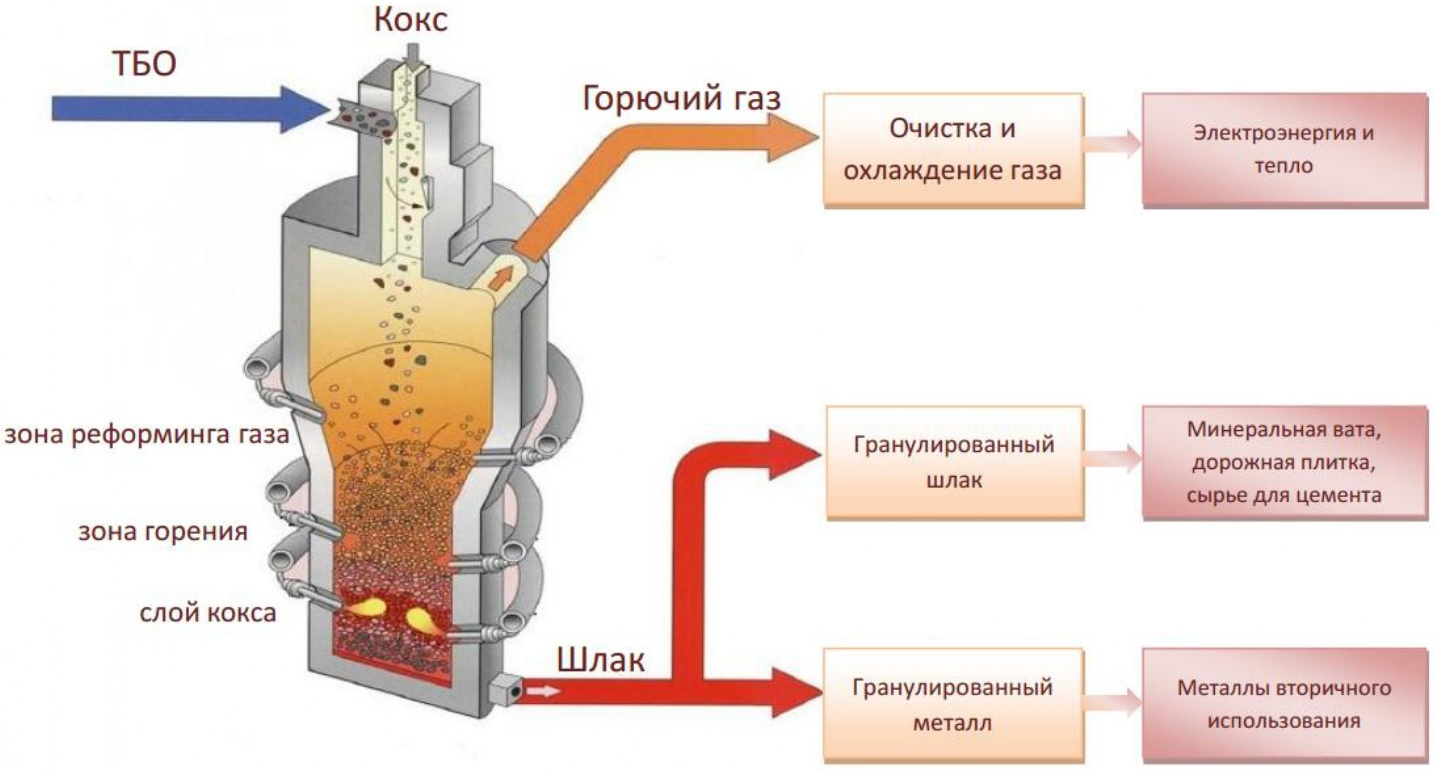
\includegraphics[width=0.8\textwidth]{media/chem2/image77}
	\caption*{Рис.14 - Технологическая схема газификации}
\end{figure}

\begin{figure}[H]
	\centering
	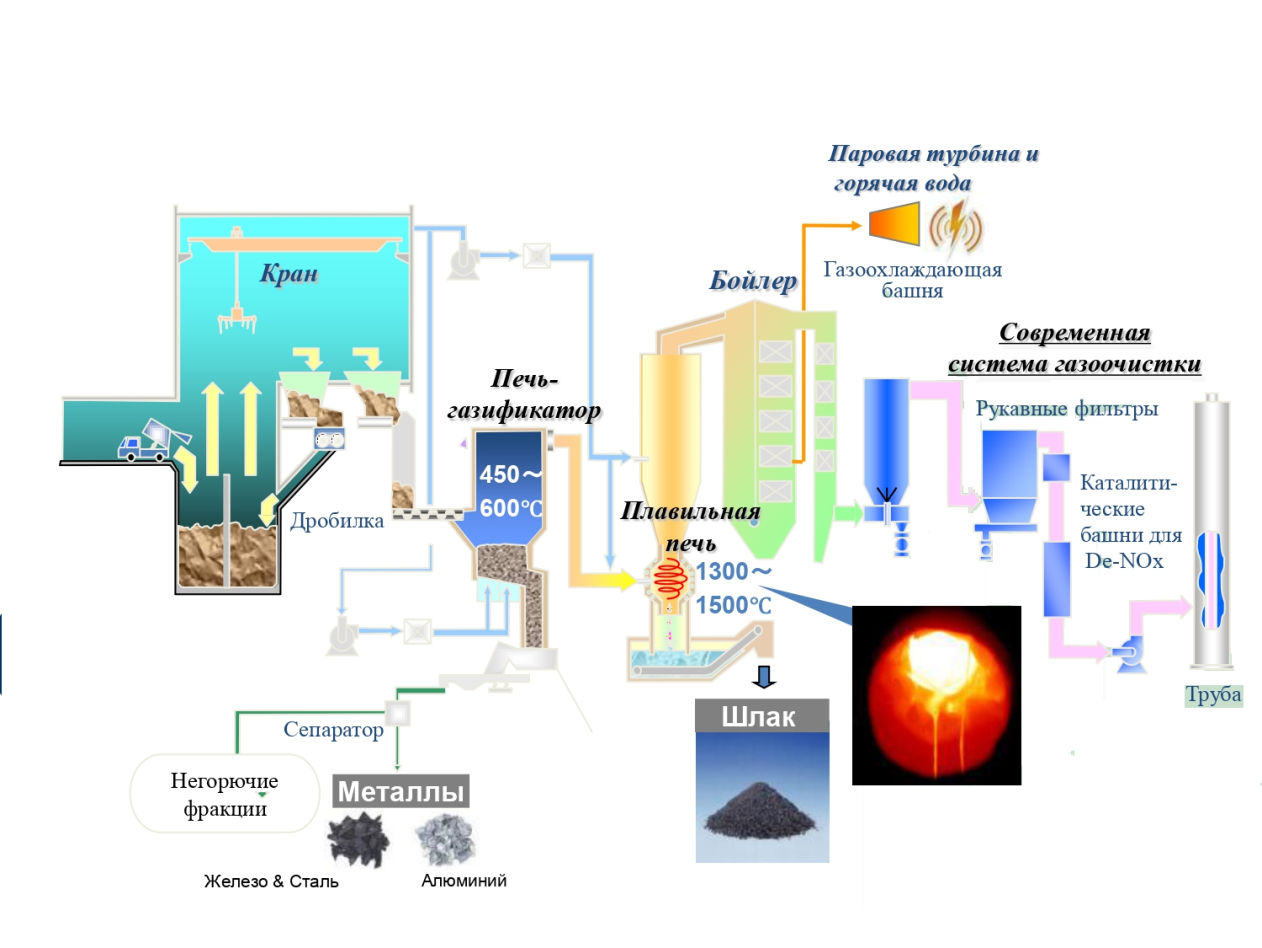
\includegraphics[width=0.8\textwidth]{media/chem2/image78}
	\caption*{Рис.15 - Технологическая схема газификации и плавления}
\end{figure}

\begin{multicols}{2}
На рисунке 15 приведена технологическая схема газификации и плавления,
используемая на заводе (компания Mitsubishi Heavy Industries, Япония). В
данном процессе на 1-м этапе производства твердое сырье (после
измельчения) подается в печь-газификатор и после сепарации получают
негорючие фракции и металлы. Далее на 2-м этапе одновременно полученный
газ из газификатора и сырье подают в плавильную печь, в которой при
высоких температурах (1300°С-1500°С) получают шлак и генераторный газ
для его дальнейшего превращения ввозобновляемые источники энергии.

По вышеуказанной технологической схеме функционирует завод по
переработке отходов потехнологии газификации и плавления, расположенный
в г.Кусиро, Япония (рисунок 16). Проект реализован компанией Mitsubishi
Heavy Indastries (Япония). Объем переработки мусора 240 тонн/сутки.
Электрическая мощность 4,6 МВт. Тип отходов: ТБО. Ввод в эксплуатацию:
2006 год.
\end{multicols}

\begin{figure}[H]
	\centering
	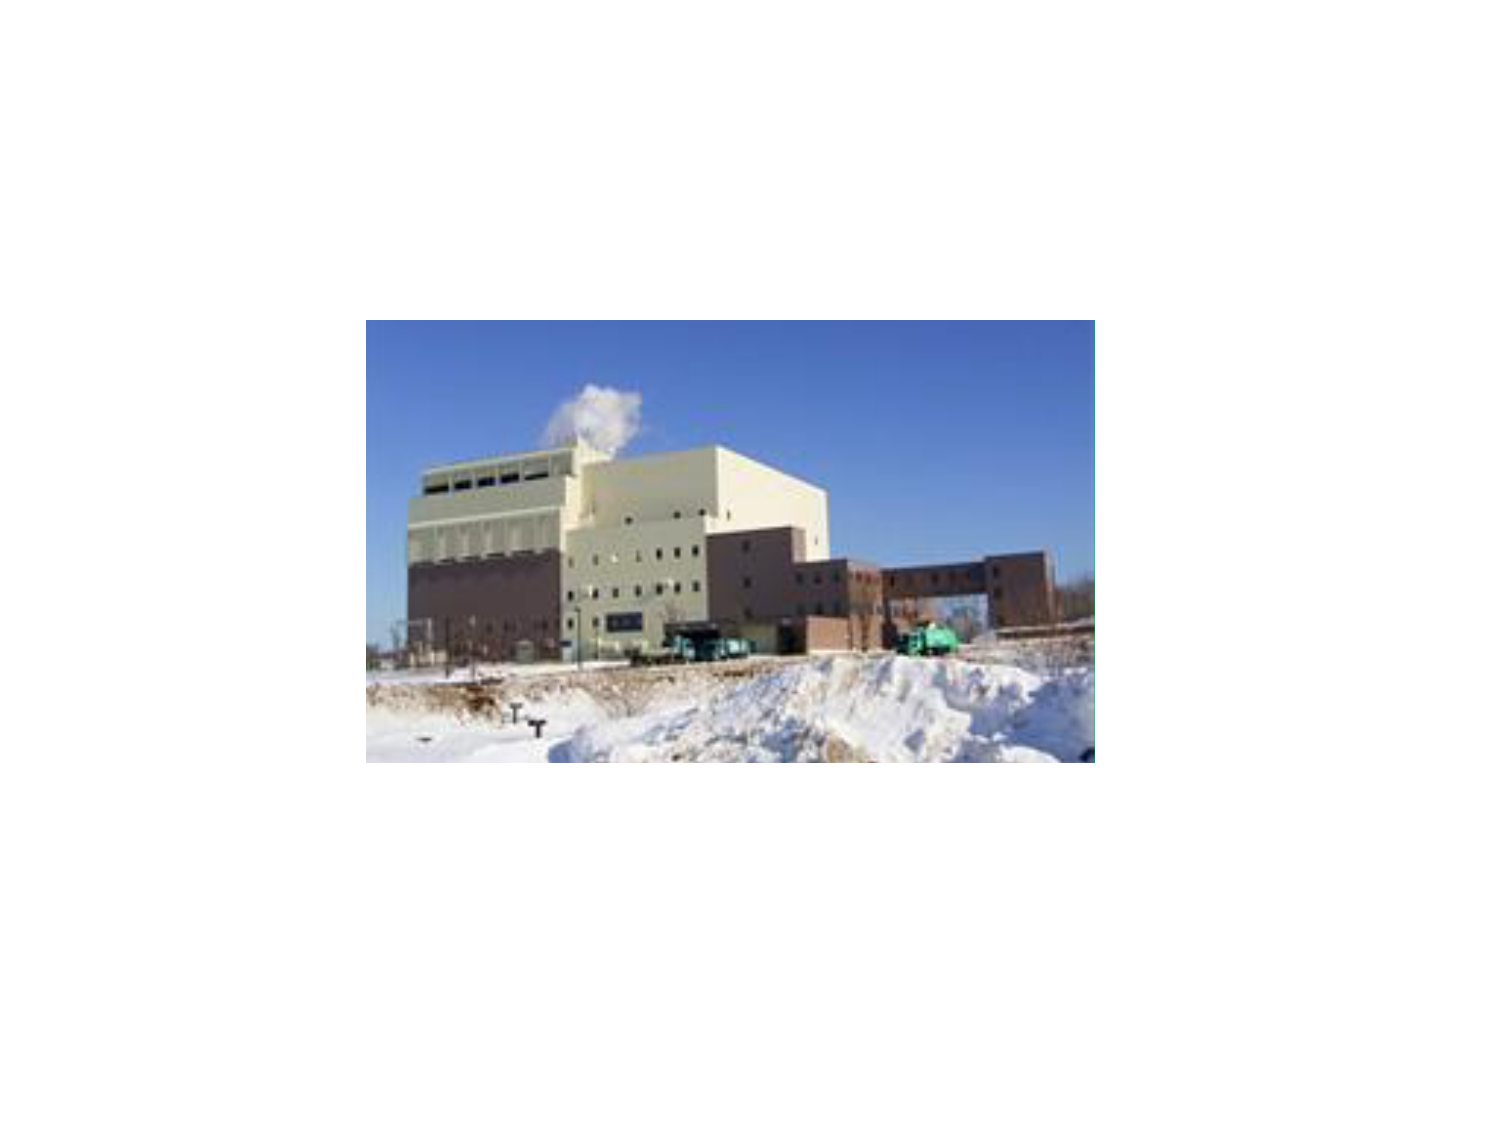
\includegraphics[width=0.8\textwidth]{media/chem2/image79}
	\caption*{Рис.16 - Завод по переработке отходов потехнологии газификации и плавления}
\end{figure}

\begin{figure}[H]
    \centering
    \begin{subfigure}[t]{0.45\textwidth}
        \centering
        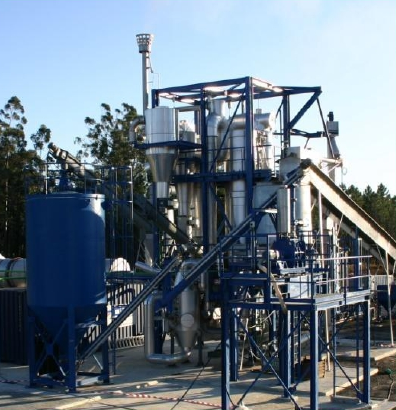
\includegraphics[width=\textwidth, height=6cm]{media/chem2/image80}
    \end{subfigure}
    \begin{subfigure}[t]{0.45\textwidth}
        \centering
        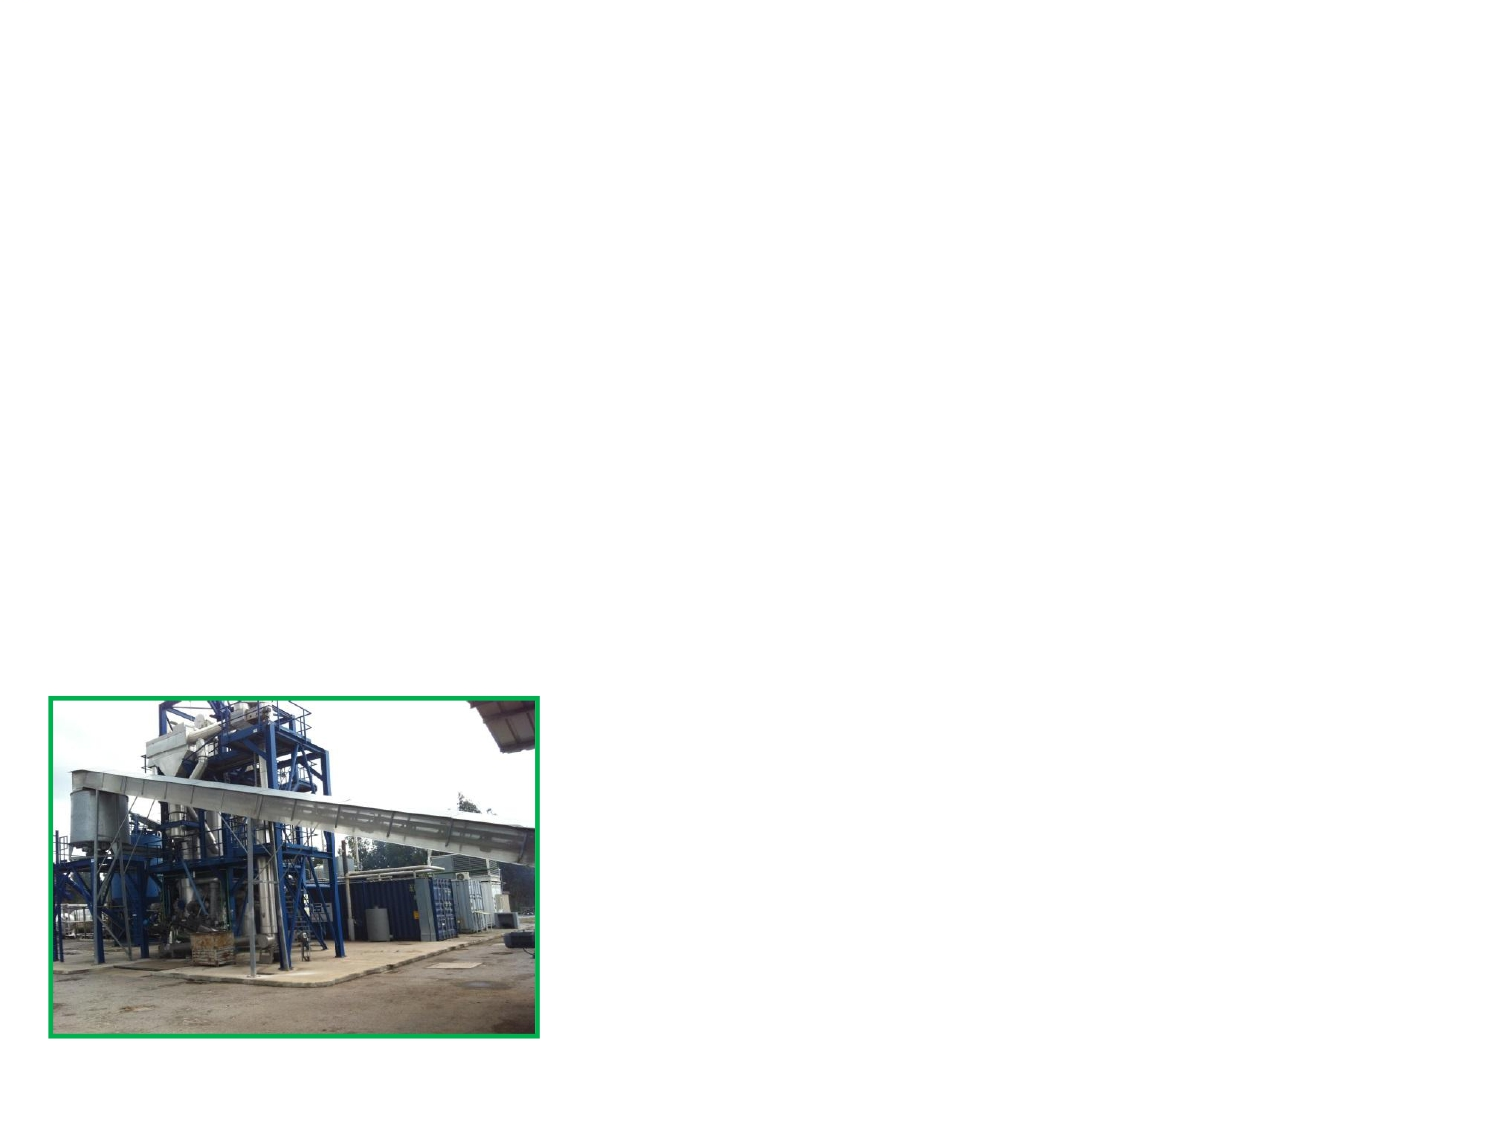
\includegraphics[width=\textwidth, height=6cm]{media/chem2/image81}
    \end{subfigure}
    \caption*{Рис.17 - Газификатор с циркулирующим кипящим слоем}
\end{figure}

\begin{multicols}{2}
Газификатор с циркулирующим кипящим слоем введен в эксплуатацию в
Португалии (Рисунок 17). Проект реализован компанией HoST Bio-Energie
(Голландия). Газификатор с циркулирующим кипящим слоем тепловой
мощностью 5 МВт, с газоочисткой и газопоршневым двигателем мощностью 1
МВт. Ввод в эксплуатацию: 2010 год. Исходным сырьем являются различные
виды топлива, такие как:сухой куриный помет 25 \%, древесная щепа 75 \%.

Схема работы установки следующая: сухая редуцированная биомасса подается
в газификатор с помощью шнека. Сырье при небольшом доступе воздуха
конвертируется при температуре около 800°C в горючий газ и затем
охлаждается до 500°C. На данном этапе происходит удаление основной части
золы и масляная очистка газа. Удаление золы перед сжиганием синтез- газа
при высокой температуре (1300-1500°C) позволяет избежать спекания золы и
обеспечивает крайний низкий уровень выбросов.

Установка не подсоединена к сетям, газ не подается на генератор для
выработки электроэнергии, хотя сам генератор имеется. Выработанный
синтез-газ сжигается при помощи факела.

Капитальные затраты на реализацию проекта составили около 6 млн. евро.
Для его реализации владельцы экспериментальной установки получили гранты
в размере 60--70 \% от общей стоимости.

В центре обезвоживания нефтяных отходов Schwarze Pumpe GmbH (Германия)
газификацию осуществляют в камерных и слоевых установках. Полученный
гене­раторный газ используется в качестве энергообеспече­ния
технологического оборудования и/или производства метанола {[}63{]}.

Финский машиностроительный концерн «Metso» про­изводит газификационные
установки для энергоснаб­жающих предприятий (например, «Lahti Energia»).
По заявлению производителей, их установка представля­ет собой новую
технологию, позволяющую с высокой эффективностью преобразовывать
предварительно обработанные отходы в энергию. Таким образом снижает­ся
потребление традиционного ископаемого топлива. Ориентировочный объем
переработки отходов на данной установке составляет от 215 до 250 тыс.
т/год {[}64{]}.

\emph{{\bfseries Технология плазменной газификации}}

На рисунке 18 приведена общая схема плазменной установки (в составе
газификатора), в которой электрический ток используется для образования
плазменной дуги, которая в свою очередь воздействует на подаваемое
сырье. Для работы плазмотронов требуются источники электропитания
(управляемые тиристорные выпрямители), трехфазные трансформаторы и др.
Согласно общей технологической схеме плазменной газификации (рисунок 18)
в настоящий момент получают электрическую и тепловую энергию. А в
перспективе продуктами плазменной газификации могут быть нефтехимические
продукты и водород.
\end{multicols}

\begin{figure}[H]
	\centering
	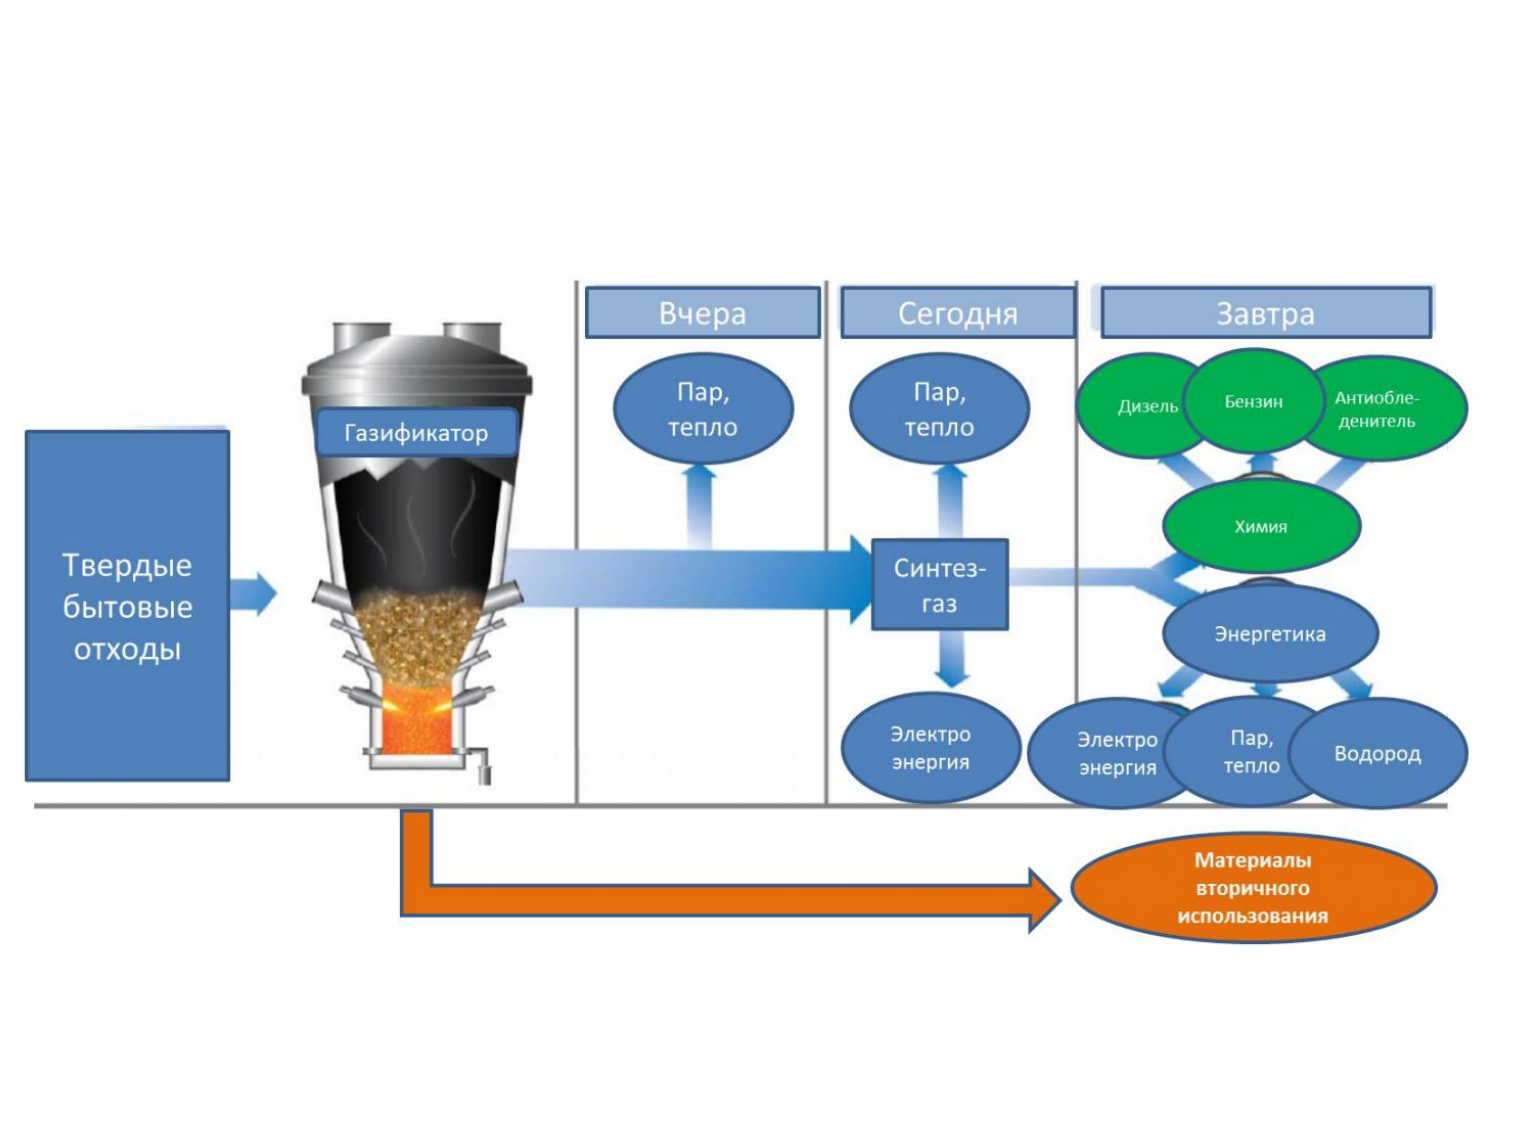
\includegraphics[width=0.8\textwidth]{media/chem2/image82}
	\caption*{Рис.18 - Общая схема плазменной газификации}
\end{figure}

\begin{figure}[H]
	\centering
	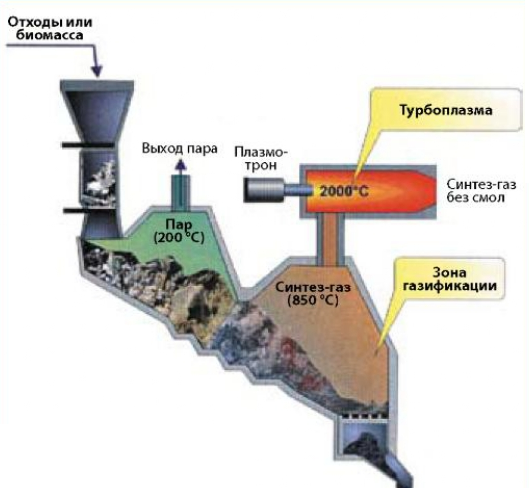
\includegraphics[width=0.7\textwidth]{media/chem2/image83}
	\caption*{Рис.19 -- Технологическая схема установки термической переработки отходов с плазменным дожигателем {[}65{]}}
\end{figure}

\begin{multicols}{2}
Плазмотроны целесообразно использовать на стадии дожигания отходящих
газов для предотвращения попадания в окружающую среду экотоксикантов
(диоксинов, фуранов, бифенилов и т.д.) (рисунок 19).

Компанией «ПЛАЗАРИУМ» (Россия) предлагается мобильная установка
плазменного уничтожения отходов под названием «PLAZARIUM MGS».
Технология заклю­чается в переработке углеродсодержащих отходов при
отсутствии свободного кислорода в плазменной струе (\textasciitilde5000
°C). При такой обработке происходит полная деструкция компонентов
отходов в синтез газ. За счет мобильного исполнения установку удобно
транспорти­ровать, размещая на шасси автомобиля, обеспечивая минимум
монтажных работ на месте с возможностью гибкой регулировки рабочих
параметров {[}66{]}. Однако высокие температуры требует большого расхода
энергии. Таким образом, сложность осуществления технологии, высокие
материальные и технические затраты, делают данную технологию
перспективой будущего.

В качестве успешного примера технологической реализации рассматриваемого
метода есть опыт американской компании Westinghouse Plasma Corporation
(WPC), которая занимается разработкой как крупных промышленных заводов,
так и небольших установок плазменной газификации. В частности, один из
заводов WPC Air Products в Великобритании позволяет ежемесячно
переработать свыше 30 килотонн мусора в виде твердых бытовых (ТБО)
промышленных и шлаковых отходов, медицинского и биологического мусора,
отходов рознично-оптовой торговли и продуктов переработки нефти. В
результате переработки завод получает очищенный синтетический газ,
используемый вкачестве энергии для электростанций, топливных элементов и
химических продуктов в виде этилового спирта, метанола, пропанола,
дизельного топлива и горючего для ракетных двигателей {[}67{]}.

Завод с технологией плазменной газификации (рисунок 20) функционирует
в г. Утасинай, Хоккайдо, Япония (рисунок 21). Проект реализован
компанией Eco Valley (Япония). Переработка -- 220 тонн/день
предварительно отсортированных отходов (2 газификационные линии, с
возможностью переработки по 110 тонн/день).
\end{multicols}

\begin{figure}[H]
	\centering
	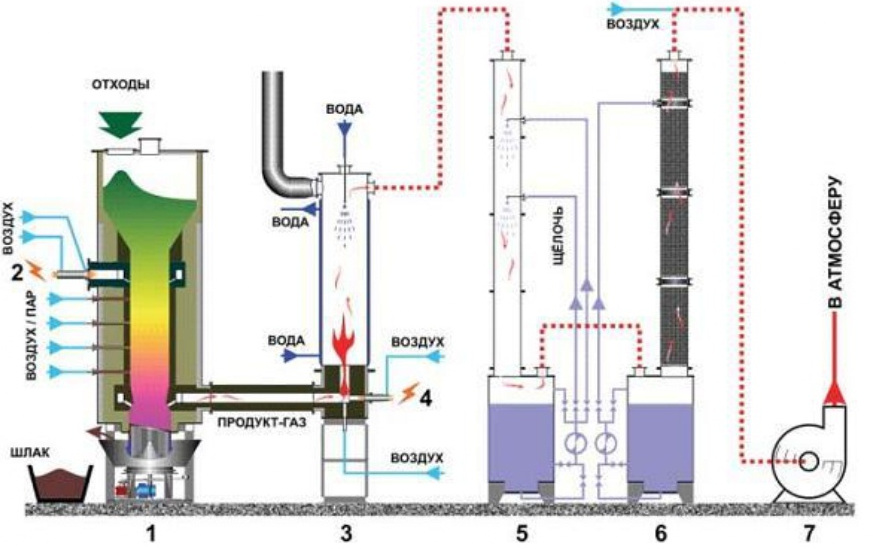
\includegraphics[width=0.8\textwidth]{media/chem2/image84}
	\caption*{Рис.20 - Техноллогическая схема плазменной установки (в составе газификатора):}
	\caption*{\normalfont\emph{1 - реактор-газификатор; 2 - генератор плазмы (до 50 кВт); 3 -
дожигатель; 4 - генератор плазмы (6 кВт); 5- скруббер распылительный; 6 - скруббер
насадочный; 7 - вытяжной вентилятор}}
\end{figure}

\begin{figure}[H]
    \centering
    \begin{subfigure}[t]{0.45\textwidth}
        \centering
        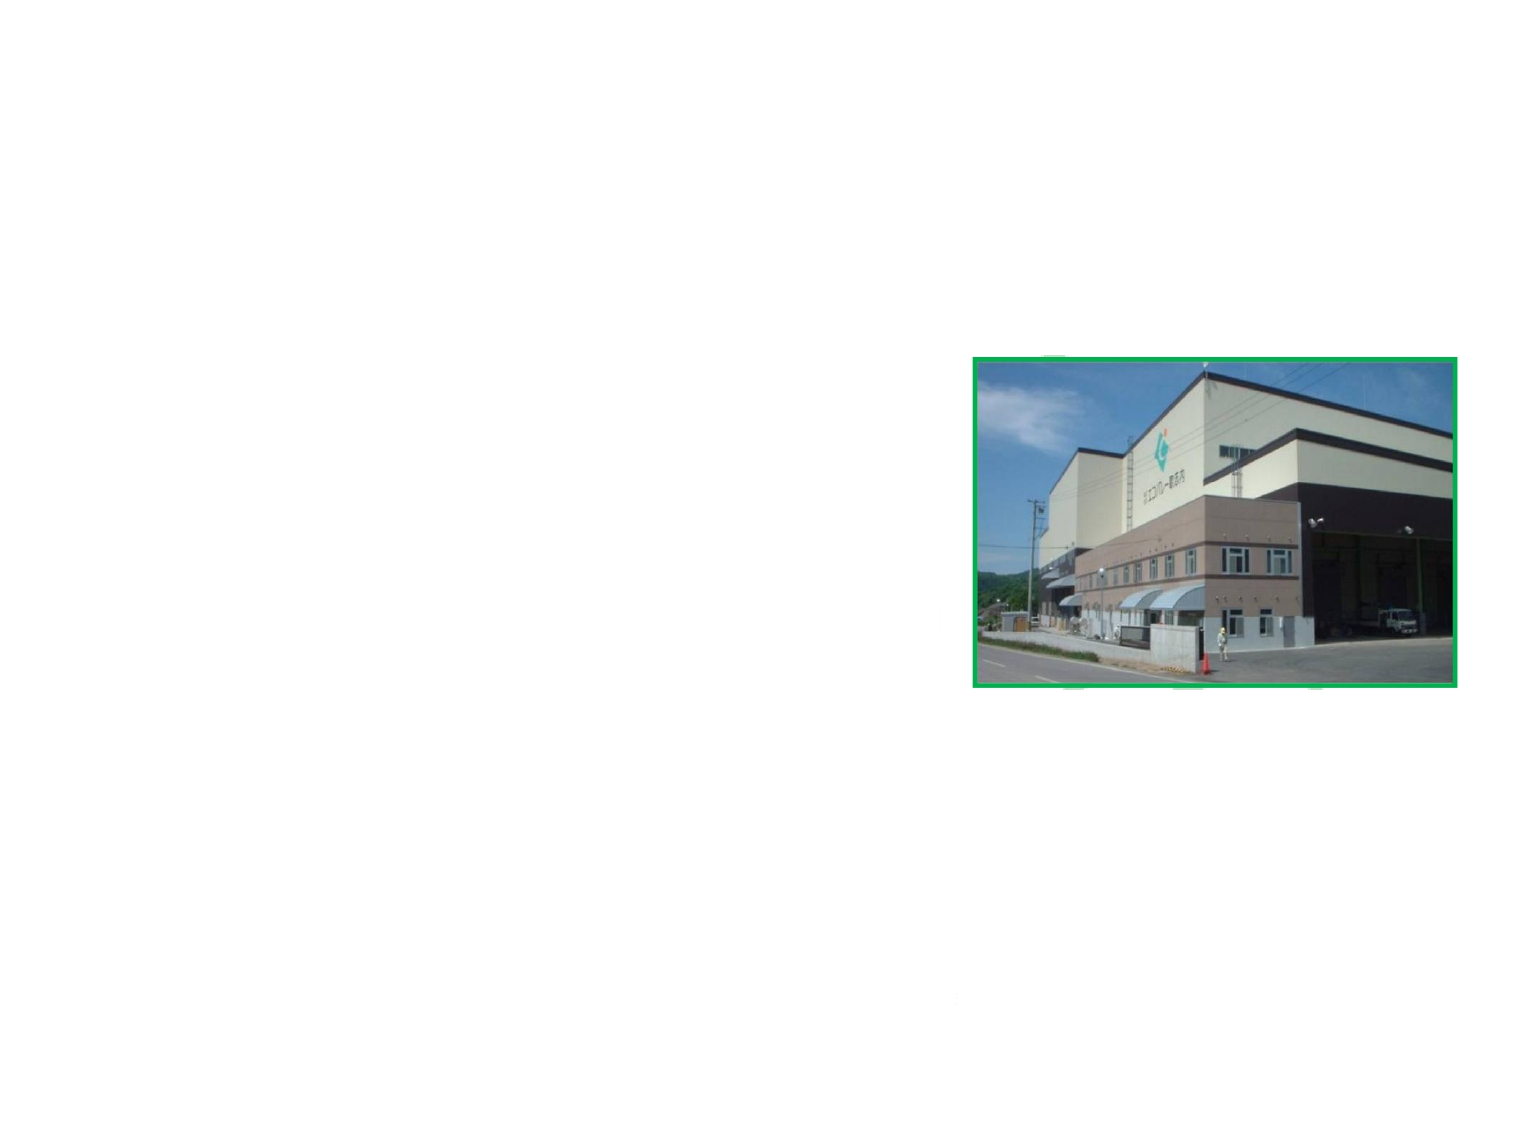
\includegraphics[width=\textwidth, height=6cm]{media/chem2/image85}
    \end{subfigure}
    \begin{subfigure}[t]{0.45\textwidth}
        \centering
        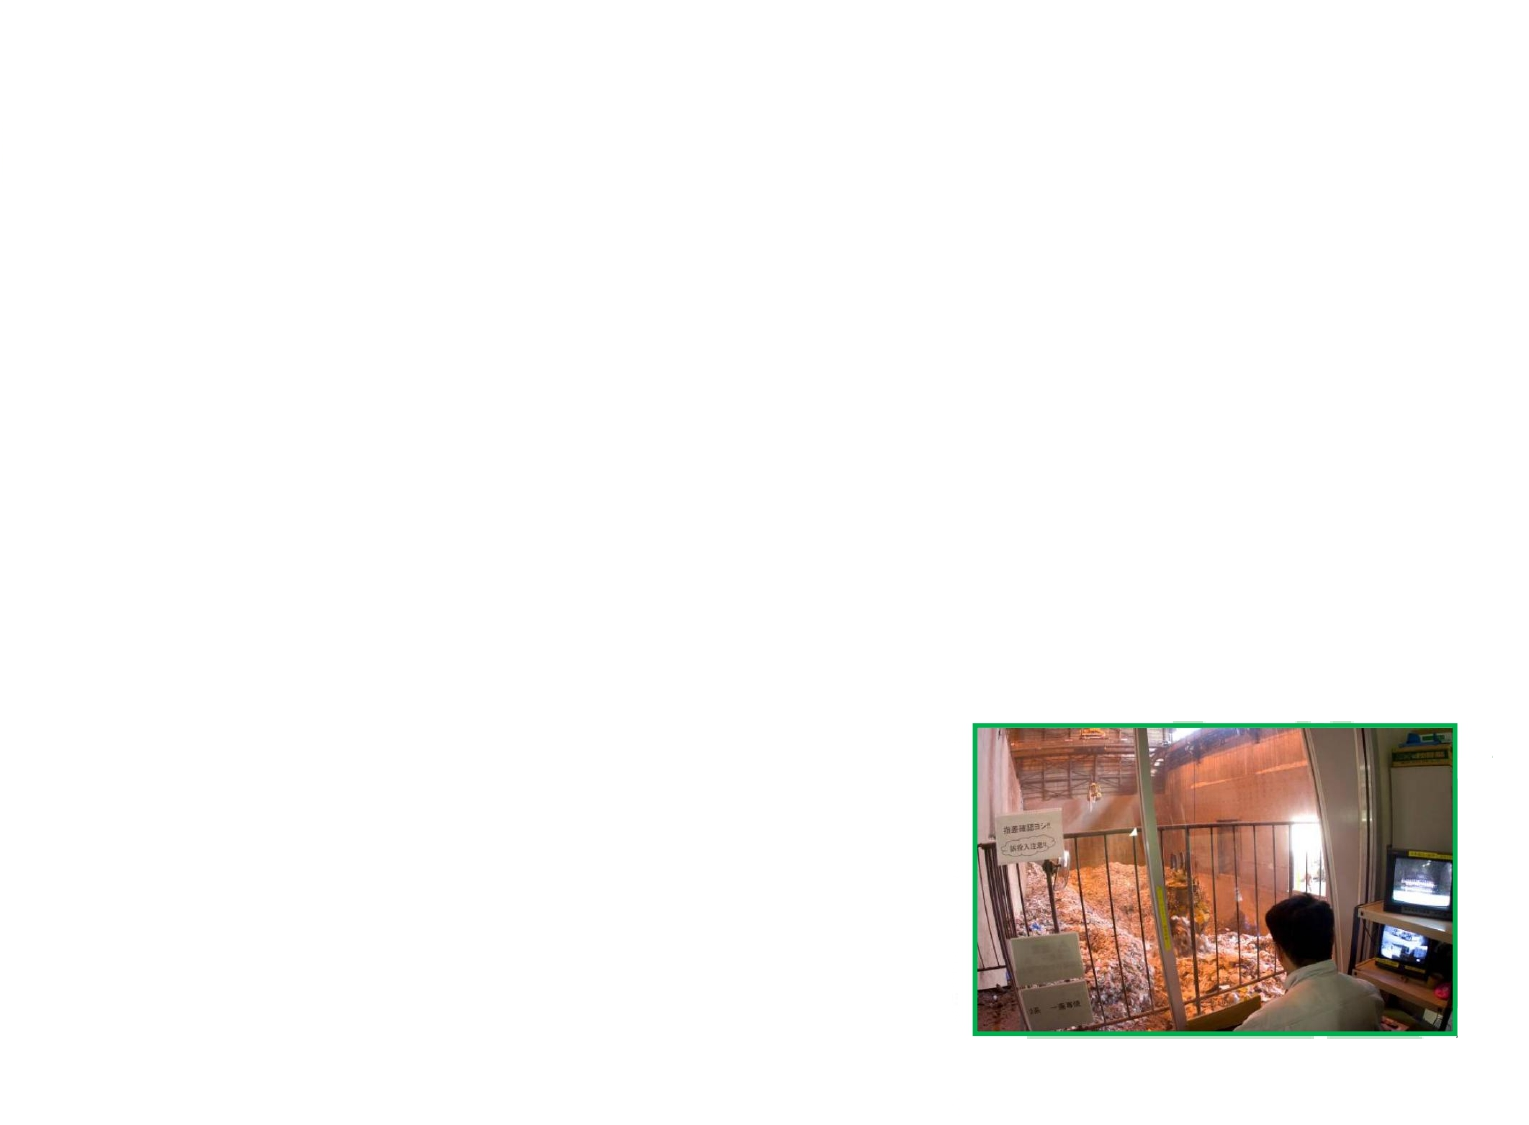
\includegraphics[width=\textwidth, height=6cm]{media/chem2/image86}
    \end{subfigure}
    \caption*{Рис.21 - Завод с технологией плазменной газификацией (г. Утасинай, Хоккайдо, Япония)}
\end{figure}

В таблице 3 для примера приведены экономические показатели строительства
комплекса по переработке отходов производства и потребления с
возможностями плазменной газификации {[}68{]}.

\tcap{Таблица 3 - Экономические показатели строительства комплекса по переработке отходов с возможностями плазменной газификации}
\begin{longtblr}[
  label = none,
  entry = none,
]{
  width = \linewidth,
  colspec = {Q[402]Q[292]Q[119]Q[123]},
  rows = {font = \small},
  row{1} = {c},
  hlines,
  vlines,
}
Параметры комплекса & Срок строительства & Общий размер инвестиций & Период возврата инвестиций\\
{Переработки промышленных и бытовых отходов 1500 тонн в сутки\\Выработки и передача потребителям электроэнергии 50 МВт∙ч\\Производства стекловидного шлака для изготовления блоков утепления из минеральной ваты 300 тонн в сутки\\Восстановление металлов 150 тонн в сутки\\Производство серы 1,5 тонны в сутки} & 24 месяца – подконтрольная эксплуатация; 6 месяцев, параллельными этапами & 307,5 млн. дол. & 5,6 лет
\end{longtblr}

\begin{multicols}{2}
В работе {[}69{]} представлено коммерческое предложение по применению
плазменной газификации для утилизации твёрдых коммунальных отходов,
осадков сточных вод, золошлаковых отходов, медицинских отходов вне
зависимости от их морфологического состава. Технология основана на
высокотемпературном (1300-1700 °С) плазмохимическом воздействии и полном
разложении утилизируемых продуктов с помощью дуговой плазмы с получением
синтез-газа, а также инертного шлака, который можно использовать как
строительный материал.

Технологические и экономические характеристики данной установки:

- производительность: газификации ТКО - 16 тыс.т/год;
высокотемпературной утилизации медицинских отходов - 1,2 тыс.т/год;
высокотемпературной минерализации опасных промышленных органических
отходов -- 0,8 тыс.т/год;

- потребляемая мощность: 6000 Вт;

- габариты установки (комплекса): 6х2х2 м, вес не более 300 кг;

- себестоимость производства единицы комплекса: 800 млн. руб.;

- требуемые затраты на НИОКР: 1500 млн. руб.;

- планируемое количество введенных в эксплуатацию комплексов в России: к
2025 году - 3 шт.; к 2030 году - до 20 шт.

Технологическое решение позволяет создание мусоросжигающих комплексов
разной мощности на основе типового оборудования.

\emph{{\bfseries Сравнительный анализ технологий переработки отходов}}

В таблице 4 представлены сравнительные характеристики основных
технологий переработки отходов, используемых в настоящее время. Видно,
что наименее экологичной технологией является сжигание, где образуется
много смол и фуранов, токсичной смолы (30 \%) и высокие выбросы дымовых
газов, а также невысокий объем разрушения отходов (70 \%), по сравнению
с другими рассматриваемыми технологиями. В последних образуется меньше
вредных выбросов и разрушение отходов составляет 90 \%. Кроме того,
процесс сжигания наряду с обычной газификацией требует сортировки
отходов и в этих процессах в основном получают электрическую и тепловую
энергию, в отличие от пиролиза и плазменной газификации, в которых можно
получить дополнительно еще синтез-газ и жидкие топлива.

Таким образом, учитывая вышеизложенное, следует выделить пиролиз и
плазменную газификацию, позволяющие получать наибольшее количество
ценных продуктов (с относительно невысокими выбросами вредных веществ) и
др. Ниже приведены основные преимущества и недостатки плазменной
газификации по сравнению с другими известными технологиями утилизации.
Основные преимущества:

\end{multicols}

\tcap{Таблица 4 - Сравнительный анализ технологий переработки отходов}
\begin{longtblr}[
  label = none,
  entry = none,
]{
  width = \linewidth,
  colspec = {Q[198]Q[254]Q[210]Q[275]},
  cells = {c},
  hlines,
  vlines,
}
{~\\\textbf{Сжигание}} & \textbf{Пиролиз			и термическое разложение без доступа			кислорода} & {~\\\textbf{Обычная			газификация}} & \textbf{Плазменная			газификация с использованием воздушной			плазмы}\\
{
			70
			\% разрушение
			\\(650\textsuperscript{о}С			)} & {
			90
			\% разрушение
			\\(450			– 900 \textsuperscript{о}С			)} & {
			90
			\% разрушение
			\\(800			\textsuperscript{о}С)} & Полное			разрушение (2000 \textsuperscript{о}С)\\
Много
			смол и фуранов & Есть
			смолы и фураны & Есть
			смолы и фураны & Нет
			смол и фуранов\\
30
			\% токсичной смолы & 10
			\% золы & 10
			\% золы & Нет
			золы\\
Кроме
			отдельных видов неорганических отходов & Кроме
			отдельных видов неорганических отходов & Кроме
			отдельных видов неорганических отходов & Любой
			вид отходов\\
Требуется
			сортировка отходов & Требует
			однородного состава  в течение года & Требуется
			сортировка отходов & Не
			требуется сортировка отходов\\
Большой
			объем отходов & Малый
			объем отходов & Малый
			объем отходов & Большой
			объем отходов\\
Высокие
			выбросы дымовых газов & Средние
			выбросы дымовых газов & Средние
			выбросы дымовых газов & Очень
			низкие выбросы дымовых газов\\
Чувствителен
			к влажности отходов & Чувствителен
			к влажности отходов & Чувствителен
			к влажности отходов & Не
			чувствителен к влажности отходов\\
Генераторный
			газ (технический) & Забалластированный
			синтез-газ & Генераторный
			газ (технический) & Высокое
			качество получаемого синтез-газа\\
Выход:
			тепло, электроэнергия & Выход:
			Синтез-газ, жидкие топлива, электроэнергия,
			тепло & Выход: тепло, электроэнергия & Выход:
			Синтез-газ, жидкие топлива,
			электроэнергия,тепло
\end{longtblr}

\begin{multicols}{2}
- возможность термически переработать (сжечь) фактически все известные
токсичные вещества;

- существенное (почти в 300 раз) и недостижимое при других способах
утилизаци и уменьшение первоначального объема отходов;

- исключение синтеза вторичных высокотоксичных веществ (диоксинов), при
наличии в отходах хлорсодержащих веществ за счет высокой температуры
плазменного воздействия (2000 °С), а также существенно меньшее, чем у
других технологий содержание NO\textsubscript{x}, SO\textsubscript{x} и
CO\textsubscript{2} в отходящих газах;

- за счет высокой степени радикального разделения веществ и газификации
углерода и водорода достигается минимальное содержание золы и пыли,
выбрасываемых в окружающую среду;

Отметим, однако, и основные недостатки технологии:

- большое энергопотребление (до 1 МВт), необходимое для эксплуатации
плазменного генератора;

- отходы желательно измельчить (размер <100 мм) для лучшей
газификации или предварительно газифицировать;

- высокие инвестиционные затраты по сравнению с другими технологиями
приводит к более длительному сроку окупаемости.

Помимо упомянутого высокого энергопотребления плазменных генераторов
(плазмотронов) сдерживающими факторами являются также ряд проблем,
связанных с надежностью и сложностью их работы и управления, а также
относительно быстрым изнашиванием электродов (до 100 часов). Наиболее
часто в таких технологиях используются СВЧ-плазмотроны переменного тока,
применяемые для нагрева среды в плазмохимических реакторах. Однако
следует обратить внимание на сложность управления такими плазмотронами.

Далее приведем основные преимущества и недостатки технологии пиролиза.
Основные преимущества пиролиза:

- отсутствие вредных выбросов в атмосферу (по срав­нению со сжиганием);

- переработка сырья с высокой зольностью (уменьше­ние объема исходного
сырья), минимальное загрязнение конечных веществ;

- возможность получения полезных продуктов для химической и
энергетической промышленностей;

- низкая требовательность к качеству исходного сырья, в результате чего
практически не требуется предвари­тельная обработка.

К недостаткам пиролиза следует отнести:

- сложность конструкции реакторных устройств;

- дороговизна оборудования.

{\bfseries Выводы.} В настоящее время особенно актуальным в Казахстане
является разработка отечественной экологичной технологии безотходной
утилизации с учетом имеющихся решений для внедрения в промышленность.
Анализ нынешней ситуации в Казахстане в области переработки отходов
показал, что еще не решен вопрос вторичного использования или утилизации
бытовых и органических отходов, а их объемы ежегодно растут очень
быстро. Результаты исследования показали, что сжигание отходов
представлено как широко применяемая, но сопряженная с высокими выбросами
загрязняющих веществ технология. Пиролиз, напротив, обладает большим
потенциалом при переработке органических и полимерных отходов, так как
позволяет получать ценное жидкое и газообразное топливо, а также
позволяет снизить выбросы парниковых газов, что особенно важно для
выполнения Казахстаном обязательств в рамках Парижского соглашения по
климату.

Газификация, как более сложный процесс, открывает перспективы для
высокоэффективного получения синтез-газа, но требует точного контроля
параметров и более высокой технологической оснащенности. В связи с этим,
назревает острый вопрос необходимости развития данного научного
направления по утилизации отходов, которая может обеспечить качественное
изменение потребительских свойств продукции и избежать прямого сжигания
сырья для уменьшения вредных выбросов. В связи с различными
характеристиками отходов для каждого их вида необходимо проведение
анализа сырьевой базы, исследования образцов, разработка технологической
схемы производства, материально-тепловых балансов производства,
экономических оценок. В социально-экономическом плане главным является
извлечение максимальной прибыли предприятиями, занятыми в данной сфере.
Таким образом, необходим комплексный подход, для чего следует
одновременно рассматривать концепции защиты окружающей среды,
энергосбережения и сокращения потребления, а также необходима
государственная поддержка, что в перспективе позволит создать устойчивую
систему управления отходами.

\emph{{\bfseries Финансирование.}Настоящая работа выполнена при финансовой
поддержке Комитета науки Министерства науки и высшего образования
Республики Казахстан (№ BR21882171 «ЦУР 9.4: Развитие «зеленой»
экономики Казахстана путем переработки минерального сырья и отходов
методом пиролиза»).}
\end{multicols}

\begin{center}
{\bfseries Литература}
\end{center}

\begin{references}
1. Hoang, A.T., Pham, V.V., Nguyen, X.P. Integrating renewable sources
intoenergy system for smart city as a sagacious strategy towards clean
and sustainableprocess.//J. Clean. Prod.- 2021.- Vol.305. - Р.127161.
\href{https://doi.org/10.1016/j.jclepro.2021.127161}{DOI
10.1016/j.jclepro.2021.127161}.

2. Xiao S., Dong H., Geng Y., Francisco M.-J., Pan H., Wu F. An overview
of the municipal solid waste management modes and innovations in
Shanghai, China. Environ// Sci. Pollut. Control Ser. -2020.- Vol.27.-
P.29943--29953.
\href{https://doi.org/10.1007/s11356-020-09398-5}{DOI10.1007/s11356-020-09398-5}.

3. Ye Y., Ngo H.H., Guo W., Chang S.W., Nguyen D.D., Varjani S., Ding
A., Bui X.-T.,Nguyen, D.P. Bio-membrane based integrated systems for
nitrogen recoveryin wastewater treatment: current applications and
future perspectives//Chemosphere.-2020. -Vol.265.- P.129076.
\href{https://doi.org/10.1016/j.chemosphere.2020.129076}{DOI
10.1016/j.chemosphere.2020.129076}.

4. Ziadat A, Mott H. Assessing solid waste recycling opportunities for
closed campuses // Management of Env Quality. - 2005. -Vol.16(3). - P.
250-256. \href{https://doi.org/10.1108/14777830510591679}{DOI
10.1108/14777830510591679}

5. Hoang A.T., Pham, V.V., Nguyen, X.P. Integrating renewable sources
intoenergy system for smart city as a sagacious strategy towards clean
and sustainableprocess// J. Clean. Prod.- 2021. -Vol.305. - P.127161.
\href{https://doi.org/\%2010.1016/j.jclepro.2021.127161}{DOI
10.1016/j.jclepro.2021.127161}.

6. Hoang A.T., Tuan I., Nguyen H., Phuong H. Nguyen. Scrap tire
pyrolysis as a potential strategy for waste management pathway: a review
// Energy Sources, Part A: Recovery, Utilization, and Environmental
Effects. - 2020. DOI 10.1080/15567036.2020.1745336.

7. Seferlis P., Varbanov P.S., Papadopoulos A.I., Chin H.H., Klemeˇs
J.J. Sustainable design, integration, and operation for energy
high-performance processsystems//Energy.- 2021. - Vol.224- P.120158.
\href{https://doi.org/10.1016/j.energy.2021.120158}{DOI
10.1016/j.energy.2021.120158}.

8. World Bank. What a Waste: Global Review of Solid Waste Management.
-Washington: Urban Develop\-ment.- 2012.- No 15.- 98 p.

9. Themelis N., Kim Y., Brady M. Energy recovery from New York City
municipal solid wastes // Waste Management \& Research.- 2002. - Vol.
20(3).- P.223--233. DOI
\href{http://dx.doi.org/10.1177/0734242X0202000303}{10.1177/0734242X0202000303}.

10. Usmani Z., Kumar V., Varjani S., Gupta P., Rani R., Chandra A.
Chapter 11~Municipal solid waste to clean energy system: a
contribution toward sustainable development.//
\href{https://www.sciencedirect.com/book/9780444643216/current-developments-in-biotechnology-and-bioengineering}{Current
Developments in Biotech\-nology and Bioengineering}{\bfseries .-} 2020. -
Р.217-231. \href{https://doi.org/10.1016/B978-0-444-64321-6.00011-2}{DOI
10.1016/B978-0-444-64321-6.00011-2}.

11. Yang Y., Liew,R.K., Tamothran A.M., Foong S.Y., Yek P.N.Y., Chia
P.W., Tran T.V.,Peng W., Lam S.S. Gasification of refuse-derived fuel
from municipal solidwaste for energy production: a review// Environ.
Chem. Lett. -2021.-№19.- P.2127--2140.
\href{https://doi.org/10.1007/s10311-020-01177-5}{DOI
10.1007/s10311-020-01177-5}.

12. ~\href{https://ulysmedia.kz/author/21/}{Курманов Б}. Отходы в
доходы: почему в Казахстане переработка мусора превратилась в тему для
обсуждения. {[}Электронный ресурс{]}. URL:
\href{https://ulysmedia.kz/analitika/11719-otkhody-v-dokhody-pochemu-v-kazakhstane-pererabotka-musora-prevratilas-v-temu-dlia-obsuzhdeniia/}{https://ulysmedia.kz}.-Дата
обращения: 04.02.2025.

13. Горбунова А. Казахстан накопил 120 млн тонн мусора. Что с ним
делать? {[}Электронный ресурс{]} URL:
\href{https://forbes.kz/process/ecobusiness/kazahstan_nakopil_120_mln_tonn_byitovogo_musora_chto_s_nim_delat/}{https://forbes.kz}
Дата обращения 04.02.2025.

14. Алиев И. Перерабатывать отходы в энергию планируют в Казахстане.
{[}Электронный ресурс{]} URL:
\url{https://www.kp.kz/online/news/3898668//-} Дата обращения:
04.02.2025.15. Бабаева Р. Жизнь после бака: как сейчас выглядит система утилизации
отходов // РБК. Тренды. {[}Электронный ресурс{]}. URL:
\url{https://trends.rbc.ru/trends/green/cmrm/60ad10399a794783c51ea200}.-Дата
обращения: 04.02.2025.

16. Ситдиков Ж.Ж., Мессерле В.Е., Устименко А.Б., Баймулдин Р.В.
Технология переработки углеродсодержащих отходов // Вестник КазНУ. Серия
физическая.- 2017. - Т.60(1). - С.12-16.

17. Денисов В. В., Денисова И. А., Гутенев В. В., Фесенко Л. Н. Основы
инженерной экологии. Ростов н/Д: Феникс, 2013. - 623 с.
ISBN~978-5-222-21011-6

18. Beyene H.D., Werkneh A.A. Ambaye T.G. Current updates on waste to
energy (WtE) technologies: a review
//\href{https://www.sciencedirect.com/journal/renewable-energy-focus}{Renewable
Energy Focus}.- 2018. -Vol.24. -P.1-11.
\href{https://doi.org/10.1016/j.ref.2017.11.001}{DOI
10.1016/j.ref.2017.11.001}.

19. Miller Frederick C. Composting of Municipal Solid Waste and its
Components // BookMicrobiology of Solid Waste. - 2020. - P.115-154.
~ISBN 9780138747268

20. Christensen T.H., Cossu R., Stegmann R. (Eds.) 2020. Landfilling of
Waste: Biogas, firsted.CRC Press, London, United Kingdom.860 р.
\href{https://doi.org/10.1201/9781003062097}{DOI 10.1201/9781003062097}.
ISBN 9781003062097

21. Wang D., Liu X., Zeng G., Zhao J., Liu Y., Wang Q., Chen F., Li X.,
Yang Q. Understanding the impact of cationic polyacrylamide on anaerobic
digestion of waste activated sludge // Water Research. - 2018. -
Vol.130. -- P.281-290.
\href{https://doi.org/10.1016/j.watres.2017.12.007}{DOI
10.1016/j.watres.2017.12.007}.

22. Escamilla-García Raúl P.E., Camarillo-López R., Carrasco-Hernández,
Emmanuel Fernández-Rod\-ríguez, Jesús Michel Legal-Hernández. Technical
and economic analysis of energy generation from waste incineration in
Mexico // Energy Strategy Reviews. - 2020. -Vol.31:100542.
\href{https://doi.org/10.1016/j.esr.2020.100542}{DOI\\
10.1016/j.esr.2020.100542}.

23. Eilhann E.Kwon, Soosan Kim, JechanLee. Pyrolysis of waste feedstocks
in CO2 for effective energy recovery and waste treatment // Journal of
CO2 Utilization. - 2019. - Vol.31.- P.173-180.
\href{https://doi.org/10.1016/j.jcou.2019.03.015}{DOI\\
10.1016/j.jcou.2019.03.015}.

24. Phuet Prasertcharoensuk Steve, J. Bull Anh N.Phan. Gasification of
waste biomass for hydrogen production: Effects of pyrolysis parameters
// Renewable Energy. - 2019.-Vol.143. - P.112-120.
\href{https://doi.org/10.1016/j.renene.2019.05.009}{DOI
10.1016/j.renene.2019.05.009}.

25. Wan-Ting Chen, Md.Akiful Haque, Taofeng Lu, Aersi Aierzhati, Gregory
Reimonn. A perspective on hydrothermal processing of sewage sludge //
Current Opinion in Environmental Science \& Health. - 2020. - Vol.14. -
P.63-73. \href{https://doi.org/10.1016/j.coesh.2020.02.008}{DOI
10.1016/j.coesh.2020.02.008}.

26. Farooq, A., Haputta, P., Silalertruksa, T., Gheewala, S.H.A
framework for theselection of suitable waste to energy technologies for
a sustainable municipal solidwaste management system. Fron.
Sustain.-2021.- Vol.2. - Р.27.
\href{https://doi.org/10.3389/frsus.2021.681690}{DOI
10.3389/frsus.2021.681690}.

27. Cheng Hu Y. Municipal solid waste (MSW) as a renewable source of
energy: Current and future practices in China // Bioresource Technology.
- 2010.-Vol.101(11).- P.3816 - 3824.
\href{https://doi.org/10.1016/j.biortech.2010.01.040}{DOI \\10.1016/j.biortech.2010.01.040}

28. Sharholy M, Ahmad K, Vaishya R, Gupta R. Municipal solid waste
characteristics and management in Allahabad, India//Waste Management.-
2007. -Vol.27(4)-P.490-496.
\href{https://doi.org/10.1016/j.wasman.2006.03.001}{DOI
10.1016/j.wasman.2006.03.001}

29. Ahmed A. Environmental Properties of Waste and By Product Materials
Used in Constructions // J solid waste techno mgmt. -2014.-Vol.40, № 2.
- P.160-169. \href{https://doi.org/10.5276/JSWTM.2014.160}{DOI
10.5276/JSWTM.2014.160}

30. Mickael D. Categorization and Sorting for Waste Management // Int.
J. Waste Resour. - 2016. - Vol.6(2). DOI
\href{http://dx.doi.org/10.4172/2252-5211.1000227}{10.4172/2252-5211.1000227}

31. Jones A, Harrison R. Emission of ultrafine particles from the
incineration of municipal solid waste//A review. Atmospheric
Environment.-2016.-Vol.140.-P.519-528.
DOI 10.1016/j.atmosenv.2016.06.005

32. Gutberlet J. Waste, poverty and recycling //Waste
Management.-2010.-Vol.30(2).- P.171-173 DOI
\href{http://dx.doi.org/10.1016/j.wasman.2009.11.006}{10.1016/j.wasman.2009.11.006}

33. Умарова М. Добиться стопроцентной переработки золоотходов
предлагают в
Казахстане. URL: \href{http://agmpportal.kz/dobitsya-stoprotsentnoj-pererabotki-zoloothodov-predlagayut-v-kazahstane\%20/}{http://agmpportal.kz}.- Дата обращения: 05.02.2025.

34. Luke Makarichi, Warangkana Jutidamrongphan, Kua-ananTechato. The
evolution of waste-to-energy incineration: A review // Renewable and
Sustainable Energy Reviews.- 2018.-Vol.91.-P.812-821.
\href{https://doi.org/10.1016/j.rser.2018.04.088}{DOI
10.1016/j.rser.2018.04.088}.

35. Xueliang Yuan, Xiaohan Fan, Jiaxin Liang, Mengyue Liu, Yuqiang Teng,
Qiao Ma, Qingsong Wang, Ruimin Mu, Jian Zuo. Public Perception towards
Waste-to-Energy as a Waste Management Strategy: A Case from Shandong,
China // Int. J. Environ. Res. Public Health 2019.- Vol.16(16). -
P.2997. \href{https://doi.org/10.3390/ijerph16162997}{DOI
10.3390/ijerph16162997}.

36. Caiyun Cui, Yong Liu, Bo Xia, Xiaoyan Jiang, Martin Skitmore.
Overview of public-private partnerships in the waste-to-energy
incineration industry in China: Status, opportunities, and challenges //
Energy Strategy Reviews.- 2020.- Vol.32:100584.
\href{https://doi.org/\%20DOI\%2010.1016/j.esr.2020.100584}{DOI
10.1016/j.esr.2020.100584}

37. Chen X., Lin, J., Li X., Ma Z. A novel framework for selecting
sustainablehealthcare waste treatment technologies under Z-number
environment//J. Oper. Res.Soc.- 2020.- Vol.72 (9).- P.1-14.
\href{https://doi.org/10.1080/01605682.2020.1759382}{DOI\\
10.1080/01605682.2020.1759382}.

38. Richard L. Skaggs, André M.Coleman, Timothy E.Seiple, Anelia
R.Milbrandt. Waste-to-Energy biofuel production potential for selected
feedstocks in the conterminous United States // Renewable and
Sustainable Energy Reviews.-2018.-Vol.82.- P.2640-2651.
\href{https://doi.org/10.1016/j.rser.2017.09.107}{DOI
10.1016/j.rser.2017.09.107}.

39. Amen R., Hameed J., Albashar G., Kamran H.W., Hassan Shah M.U.,
Zaman M.K.U., Mukhtar A., Saqib, S., Ch,S.I., Ibrahim M., Ullah, S.,
Al-Sehemi A.G., Ahmad S.R.,Klemeˇs J.J., Bokhari, A., Asif S., Modelling
the higher heating value ofmunicipal solid waste for assessment of
waste-to-energy potential: a sustainable
casestudy//J.Clean.Prod.-2021.-Vol.287:P.125575.
\href{https://doi.org/10.1016/j.jclepro.2020.125575}{DOI
10.1016/j.jclepro.2020.125575}.

40. Hu G. Li, J., Zeng G. Recent development in the treatment of oily
sludge from petroleum industry: a review//Journal of Hazardous
Materials.-2013.- Vol.261.- P.470-490.
\href{https://doi.org/10.1016/j.jhazmat.2013.07.069}{DOI
10.1016/j.jhazmat.2013.07.069}

41. De Medeiros A. D. M., da Silva Junior C. J. G., de Amorim,J. D. P.
Oily wastewater treatment: methods, challenges, and trends// Processes.-
2022. - Vol.10(4). - P.743. DOI
\href{http://dx.doi.org/10.3390/pr10040743}{10.3390/pr10040743}

42. Коленчуков О.А., Башмур К.А., Агафонов Е.Д., Бухтояров В.В.,
Сергиенко Р.Б. Анализ современных технологий переработки и утилизации
углеводородных отходов термическими способами // SOCAR
Proceedings.-2023. - № 2. - Р.127-137. DOI 10.5510/OGP20230200855

43. Петровский Э. А., Соловьев Е. А., Коленчуков О. А. (2018).
Современные технологии переработки нефтешла­мов // Вестник БГТУ им. В.Г.
Шухова.-2018.- №4 - С.124-132. DOI \\
10.12737/article\_5ac24a32b29f22.54931659

44. Сарыглар Ч.А., Чысыма Р.Б. Основные направления переработки угля //
Фундаментальные иссле\-дования - 2018. -№ 11.- С.121-127.
DOI~\href{https://doi.org/10.17513/fr.42311}{10.17513/fr.42311}

45. Исламов С.Р., Степанов С.Г. Глубокая переработка угля: введение в
проблему выбора технологии // Уголь.- 2007. - № 10 (978). - С.53--58.

46. Пиролиз каменного угля: понятие и продукты {[}Электронный ресурс{]}.
URL:
\href{https://ztbo.ru/o-tbo/stati/piroliz/piroliz-kamennogo-uglya-ponyatie-i-produkti}{https://ztbo.ru} .-Дата
обращения: 06.02.2025).

47. Шантарин В.Д. Безальтернативный метод утилизации углеродосодержащих
отходов. Научное обо­зрение. Технические науки.- 2016. -№ 2. - С.71-74.

48. Бахонина Е.И. Современные технологии переработки и утилизации
углеводородсодержащих отходов. Сообщение 1. Термические методы
утилизации и обезвреживания углеродсодержащих отходов // Башкирский
хими­ческий журналю- 2015. - № 22(1). - С.20-29.

49. Зубаиров С.Γ., Ахметов А. Ф., Байрамгулов А. С. Оценка
напряженно-деформированных состояний базовой и усовершенствованной
конструкций модулей пиролиза нефтесодержащих шламов // SOCAR
Proceedings.- 2018.- № 2.- С.71-76. DOI 10.5510/OGP20230200855

50. Копылов Н.И., Каминский Ю.Д., Куликова М.П. Пиролиз угля Тувинского
месторождения // Химическая технология.-2008.- Т.9(4). - С.168 - 173.

51. Sokolinskii S.M., Khudyakov Yu., Lapidus D.A. Calculation of a
DirectFlow Coal Gasification Process with Liquid Slag Removal//Solid
Fuel Chemistry.-2020.- Vol.54(5).- P.269-273 DOI\\
10.3103/S0361521920050092.

52. Технология плазменной газификации -- преимущества и недостатки. URL:
\href{https://vinit.com.vn/ru/технология-плазменной-газификации-п/}{https://vinit.com.vn} . -
Дата обращения: 06.02.2025.

53. Mishra A., Gautam S., Sharma T. Effect of operating parameters on
coal gasification // International Journal of Coal Science \&
Technology.- 2018.- Vol.5(5).- P.113-125. DOI
\href{http://dx.doi.org/10.1007/s40789-018-0196-3}{10.1007/s40789-018-0196-3}.

54. Е.В. Голубев, Н.Н. Кудрявцев. Переработка нефтесодержащих отходов в
едином производственном цикле // Международный научный журнал
«Альтернативная энергетика и экология».- 2012. -№ 10 (114). - С.
112-115.

55. Козловский В.А., Колясников С.А. Строительство и использование
заводов по термической переработке отходов как этап развития технологий
зеленой экономики // Экономика и управление: теория и практика. -2022.
-Т.8.(1). - С.31-36.

56. Тяглов С.Г., Козловский В.А., Колясников С.А., Харагоргиев-Тяглов
А.А. Термическая переработка отходов- эффективный способ их утилизации и
технология развития альтернативной энергетики в Российской Федерации //
Финансовые исследования.- 2022. - № 2 (75). - С.77-82. DOI
\href{https://doi.org/10.54220/finis.1991-0525.2022.75.2.007}{10.54220/finis.1991-0525.2022.75.2.007}

57. Тугов А. Н. Исследование процессов и технологий энергетической
утилизации бытовых отходов для разработки отечественной ТЭС на ТБО:
автореф. дис. докт. техн. наук. М., 2012. - 21 с.

58. Waste-to-energy facility to be constructed in Scotland {[}Electronic
source{]}. -- URL:\\
\href{http://www.energyglobal.com/other-renewables/27102021/waste-to-energy-facility-to-be-constructed-in-scotland}{http://www.energyglobal.com}.
-- Date of access: 06.02.2025.

59. Севостьянова М.А., Соловьев Е.А. Технологическая установка для
переработки отходов нефти и нефтепродуктов методом низкотемпературного
пиролиза // Электронный сборник материалов Международной конференции
студентов, аспирантов и молодых ученых «ПРОСПЕКТ СВОБОДНЫЙ-2016»,
посвященной году образования в содружестве независимых государств,
Красноярск, Сибирский федеральный университет, 15-25 апреля 2016 г. - С.
44 - 46.

60. Хуснутдинова И.Ш., Сафиулина, А.Г., Заббаров Р.Р., Хуснутдинов С.И.
Методы утилизации нефтя­ных шламов//Известия ВУЗ. Серия: химия и
химическая технология.- 2015. № 58(10). - С.3-20.

61. Янковой Д. С., Ладыгин К. В., Стомпель С. И., Уткина Н. Н. Новая
технология утилизации нефтеш­ламов//Экология производства.-2014.- № 9. -
С.47-51.

62. Вайнштейн Э. Ф. (2003). Способ переработки органических веществ.
Патент РФ 2201951.

63. Лотош В.Е. Переработка отходов природопользования. Екатеринбург:
Полиграфист, 2007. - 503 с. ISBN 5-88425-216-1

64. Калютик А. А., Трещев,Д. А., Поздеева Д. Л. Утилизация твердых
бытовых отходов на ТЭЦ г. Санкт- Петербурга //Энергетика и
электротехника.-2019.- № 25(3). - С.59-70. DOI: \\10.18721/JEST.25304

65. Плазменная технология утилизации отходов. {[}Электронный ресурс{]}.
URL:
\href{https://betosteel.ru/articles/plazmennaya-texnologiya-utilizacii-otxodov.html}{https://betosteel.ru}.-
Дата обращения 08.02.2025.

66. Гибридный плазменный завод, модернизация установок пиролиза и
ректификации с получением топлива. PLAZARIUM MPS {[}Электронный
ресурс{]}. URL:
\href{https://www.plazarium.com/ru/products/plasma-pyrolysis-units/plazarium-mps/}{https://www.plazarium.com}.
Дата обращения: 08.02.2025.

67. Поляков М. Д., Сычев Э. В. Социальные аспекты рациональной
утилизации и переработки мусора в городском хозяйстве // Социальная
антропология города: культурное, социальное и хозяйственное пространство
: сборник научных трудов по материалам конференции, Санкт-Петербург,
21--22 марта 2019 года. СПб.: L-Print, 2019. - С.40--44.

68. Кадерлеев М. К. Технология плазменной газификации Westinghouse
Plasma Corporation {[}Электронный ресурс{]}. URL:
\href{http://www.cleandex.ru/articles/2016/03/07/zavody_po_pererabotke_othodov_proizvodstva_i_potrebleniya_v_elektroenergiyu}{http://www.cleandex.ru}.-Дата
обращения: 08.02.2025.

69. Гильмундинов. Отчет о работе. Выполнение маркетинговых исследований
(оценка рынка в России и мире, аналоги, компании ̶ конкуренты),
Новосибирск, 2021.
\end{references}

\begin{center}
{\bfseries References}
\end{center}

\begin{references}
1. Hoang, A.T., Pham, V.V., Nguyen, X.P. Integrating renewable sources
intoenergy system for smart city as a sagacious strategy towards clean
and sustainableprocess.//J. Clean. Prod.- 2021.- Vol.305. - Р.127161.
\href{https://doi.org/10.1016/j.jclepro.2021.127161}{DOI
10.1016/j.jclepro.2021.127161}.

2. Xiao S., Dong H., Geng Y., Francisco M.-J., Pan H., Wu F. An overview
of the municipal solid waste management modes and innovations in
Shanghai, China. Environ// Sci. Pollut. Control Ser. -2020.- Vol.27.-
P.29943--29953.
\href{https://doi.org/10.1007/s11356-020-09398-5}{DOI10.1007/s11356-020-09398-5}.

3. Ye Y., Ngo H.H., Guo W., Chang S.W., Nguyen D.D., Varjani S., Ding
A., Bui X.-T.,Nguyen, D.P. Bio-membrane based integrated systems for
nitrogen recoveryin wastewater treatment: current applications and
future perspectives//Chemosphere.-2020. -Vol.265.- P.129076.
\href{https://doi.org/10.1016/j.chemosphere.2020.129076}{DOI
10.1016/j.chemosphere.2020.129076}.

4. Ziadat A, Mott H. Assessing solid waste recycling opportunities for
closed campuses // Management of Env Quality. - 2005. -Vol.16(3). - P.
250-256. \href{https://doi.org/10.1108/14777830510591679}{DOI
10.1108/14777830510591679}

5. Hoang A.T., Pham, V.V., Nguyen, X.P. Integrating renewable sources
intoenergy system for smart city as a sagacious strategy towards clean
and sustainableprocess// J. Clean. Prod.- 2021. -Vol.305. - P.127161.
\href{https://doi.org/\%2010.1016/j.jclepro.2021.127161}{DOI
10.1016/j.jclepro.2021.127161}.

6. Hoang A.T., Tuan I., Nguyen H., Phuong H. Nguyen. Scrap tire
pyrolysis as a potential strategy for waste management pathway: a review
// Energy Sources, Part A: Recovery, Utilization, and Environmental
Effects. - 2020. DOI 10.1080/15567036.2020.1745336.

7. Seferlis P., Varbanov P.S., Papadopoulos A.I., Chin H.H., Klemeˇs
J.J. Sustainable design, integration, and operation for energy
high-performance processsystems//Energy.- 2021. - Vol.224- P.120158.
\href{https://doi.org/10.1016/j.energy.2021.120158}{DOI
10.1016/j.energy.2021.120158}.

8. World Bank. What a Waste: Global Review of Solid Waste Management.
-Washington: Urban Develop\-ment.- 2012.- No 15.- 98 p.

9. Themelis N., Kim Y., Brady M. Energy recovery from New York City
municipal solid wastes // Waste Management \& Research.- 2002. - Vol.
20(3).- P.223--233. DOI
\href{http://dx.doi.org/10.1177/0734242X0202000303}{10.1177/0734242X0202000303}.

10. Usmani Z., Kumar V., Varjani S., Gupta P., Rani R., Chandra A.
Chapter 11~Municipal solid waste to clean energy system: a
contribution toward sustainable development.//
\href{https://www.sciencedirect.com/book/9780444643216/current-developments-in-biotechnology-and-bioengineering}{Current
Developments in Biotech\-nology and Bioengineering} .- 2020. -
Р.217-231. \href{https://doi.org/10.1016/B978-0-444-64321-6.00011-2}{DOI
10.1016/B978-0-444-64321-6.00011-2}.

11. Yang Y., Liew,R.K., Tamothran A.M., Foong S.Y., Yek P.N.Y., Chia
P.W., Tran T.V.,Peng W., Lam S.S. Gasification of refuse-derived fuel
from municipal solidwaste for energy production: a review// Environ.
Chem. Lett. -2021.-№19.- P.2127--2140.
\href{https://doi.org/10.1007/s10311-020-01177-5}{DOI
10.1007/s10311-020-01177-5}.

12. Kurmanov B. Othody v dohody: pochemu v Kazahstane pererabotka musora
prevratilas'{} v temu dlja obsuzhdenija. {[}Jelektronnyj
resurs{]}. URL:
\href{https://ulysmedia.kz/analitika/11719-otkhody-v-dokhody-pochemu-v-kazakhstane-pererabotka-musora-prevratilas-v-temu-dlia-obsuzhdeniia/}{https://ulysmedia.kz} .-Data
obrashhenija: 04.02.2025. {[}in \\Russian{]}

13. Gorbunova A. Kazahstan nakopil 120 mln tonn musora. Chto s nim
delat'? {[}Jelektronnyj resurs{]} URL:
\href{https://forbes.kz/process/ecobusiness/kazahstan_nakopil_120_mln_tonn_byitovogo_musora_chto_s_nim_delat/}{https://forbes.kz}
Data obrashhenija 04.02.2025. {[}in Russian{]}

14. Aliev I. Pererabatyvat'{} othody v jenergiju
planirujut v Kazahstane. {[}Jelektronnyj resurs{]} URL:\\
\href{https://www.kp.kz/online/news/3898668/}{https://www.kp.kz} .- Data obrashhenija: 04.02.2025.
{[}in Russian{]}

15. Babaeva R. Zhizn'{} posle baka: kak sejchas vygljadit
sistema utilizacii othodov // RBK. Trendy. {[}Jelek\-tronnyj resurs{]}.
URL:
\href{https://trends.rbc.ru/trends/green/cmrm/60ad10399a794783c51ea200}{https://trends.rbc.ru} .- Data
obrashhenija: 04.02.2025. {[}in Russian{]}

16. Sitdikov Zh.Zh., Messerle V.E., Ustimenko A.B., Bajmuldin R.V.
Tehnologija pererabotki uglerod\-soderzhashhih othodov // Vestnik KazNU.
Serija fizicheskaja.-2017. - T.60.(1). - S.12-16. {[}in Russian{]}

17. Denisov V. V., Denisova I. A., Gutenev V. V., Fesenko L. N. Osnovy
inzhenernoj jekologii. Rostov n/D: Feniks, 2013. - 623 s. ISBN
978-5-222-21011-6. {[}in Russian{]}

18. Beyene H.D., Werkneh A.A. Ambaye T.G. Current updates on waste to
energy (WtE) technologies: a review
//\href{https://www.sciencedirect.com/journal/renewable-energy-focus}{Renewable
Energy Focus}.- 2018. -Vol.24. -P.1-11.
\href{https://doi.org/10.1016/j.ref.2017.11.001}{DOI
10.1016/j.ref.2017.11.001}.

19. Miller Frederick C. Composting of Municipal Solid Waste and its
Components // BookMicrobiology of Solid Waste. - 2020. - P.115-154.
~ISBN 9780138747268

20. Christensen T.H., Cossu R., Stegmann R. (Eds.) 2020. Landfilling of
Waste: Biogas, firsted.CRC Press, London, United Kingdom.860 р.
\href{https://doi.org/10.1201/9781003062097}{DOI 10.1201/9781003062097}.
ISBN 9781003062097

21. Wang D., Liu X., Zeng G., Zhao J., Liu Y., Wang Q., Chen F., Li X.,
Yang Q. Understanding the impact of cationic polyacrylamide on anaerobic
digestion of waste activated sludge // Water Research. - 2018. -
Vol.130. -- P.281-290.
\href{https://doi.org/10.1016/j.watres.2017.12.007}{DOI
10.1016/j.watres.2017.12.007}.

22. Escamilla-García Raúl P.E., Camarillo-López R., Carrasco-Hernández,
Emmanuel Fernández-Rod\-ríguez, Jesús Michel Legal-Hernández. Technical
and economic analysis of energy generation from waste incineration in
Mexico // Energy Strategy Reviews. - 2020. -Vol.31:100542.
\href{https://doi.org/10.1016/j.esr.2020.100542}{DOI\\
10.1016/j.esr.2020.100542}.

23. Eilhann E.Kwon, Soosan Kim, JechanLee. Pyrolysis of waste feedstocks
in CO2 for effective energy recovery and waste treatment // Journal of
CO2 Utilization. - 2019. - Vol.31.- P.173-180.
\href{https://doi.org/10.1016/j.jcou.2019.03.015}{DOI\\
10.1016/j.jcou.2019.03.015}.

24. Phuet Prasertcharoensuk Steve, J. Bull Anh N.Phan. Gasification of
waste biomass for hydrogen production: Effects of pyrolysis parameters
// Renewable Energy. - 2019.-Vol.143. - P.112-120.
\href{https://doi.org/10.1016/j.renene.2019.05.009}{DOI
10.1016/j.renene.2019.05.009}.

25. Wan-Ting Chen, Md.Akiful Haque, Taofeng Lu, Aersi Aierzhati, Gregory
Reimonn. A perspective on hydrothermal processing of sewage sludge //
Current Opinion in Environmental Science \& Health. - 2020. - Vol.14. -
P.63-73. \href{https://doi.org/10.1016/j.coesh.2020.02.008}{DOI
10.1016/j.coesh.2020.02.008}.

26. Farooq, A., Haputta, P., Silalertruksa, T., Gheewala, S.H.A
framework for theselection of suitable waste to energy technologies for
a sustainable municipal solidwaste management system. Fron.
Sustain.-2021.- Vol.2. - Р.27.
\href{https://doi.org/10.3389/frsus.2021.681690}{DOI
10.3389/frsus.2021.681690}.

27. Cheng Hu Y. Municipal solid waste (MSW) as a renewable source of
energy: Current and future practices in China // Bioresource Technology.
- 2010.-Vol.101(11).- P.3816 - 3824.
\href{https://doi.org/10.1016/j.biortech.2010.01.040}{DOI \\10.1016/j.biortech.2010.01.040}

28. Sharholy M, Ahmad K, Vaishya R, Gupta R. Municipal solid waste
characteristics and management in Allahabad, India//Waste Management.-
2007. -Vol.27(4)-P.490-496.
\href{https://doi.org/10.1016/j.wasman.2006.03.001}{DOI
10.1016/j.wasman.2006.03.001}

29. Ahmed A. Environmental Properties of Waste and By Product Materials
Used in Constructions // J solid waste techno mgmt. -2014.-Vol.40, № 2.
- P.160-169. \href{https://doi.org/10.5276/JSWTM.2014.160}{DOI
10.5276/JSWTM.2014.160}

30. Mickael D. Categorization and Sorting for Waste Management // Int.
J. Waste Resour. - 2016. - Vol.6(2). DOI
\href{http://dx.doi.org/10.4172/2252-5211.1000227}{10.4172/2252-5211.1000227}

31. Jones A, Harrison R. Emission of ultrafine particles from the
incineration of municipal solid waste//A review. Atmospheric
Environment.-2016.-Vol.140.-P.519-528. DOI 10.1016/j.atmosenv.2016.06.005

32. Gutberlet J. Waste, poverty and recycling //Waste
Management.-2010.-Vol.30(2).- P.171-173 DOI
\href{http://dx.doi.org/10.1016/j.wasman.2009.11.006}{10.1016/j.wasman.2009.11.006}

33. Umarova M. Dobit' sja stoprocentnoj pererabotki
zoloothodov predlagajut v Kazahstane. URL:\\
\href{http://agmpportal.kz/dobitsya-stoprotsentnoj-pererabotki-zoloothodov-predlagayut-v-kazahstane/}{http://agmpportal.kz} .-
Data obrashhenija: 05.02.2025. {[}in Russian{]}

34. Luke Makarichi, Warangkana Jutidamrongphan, Kua-ananTechato. The
evolution of waste-to-energy incineration: A review // Renewable and
Sustainable Energy Reviews.- 2018.-Vol.91.-P.812-821.
\href{https://doi.org/10.1016/j.rser.2018.04.088}{DOI
10.1016/j.rser.2018.04.088}.

35. Xueliang Yuan, Xiaohan Fan, Jiaxin Liang, Mengyue Liu, Yuqiang Teng,
Qiao Ma, Qingsong Wang, Ruimin Mu, Jian Zuo. Public Perception towards
Waste-to-Energy as a Waste Management Strategy: A Case from Shandong,
China // Int. J. Environ. Res. Public Health 2019.- Vol.16(16). -
P.2997. \href{https://doi.org/10.3390/ijerph16162997}{DOI
10.3390/ijerph16162997}.

36. Caiyun Cui, Yong Liu, Bo Xia, Xiaoyan Jiang, Martin Skitmore.
Overview of public-private partnerships in the waste-to-energy
incineration industry in China: Status, opportunities, and challenges //
Energy Strategy Reviews.- 2020.- Vol.32:100584.
\href{https://doi.org/\%20DOI\%2010.1016/j.esr.2020.100584}{DOI
10.1016/j.esr.2020.100584}

37. Chen X., Lin, J., Li X., Ma Z. A novel framework for selecting
sustainablehealthcare waste treatment technologies under Z-number
environment//J. Oper. Res.Soc.- 2020.- Vol.72 (9).- P.1-14.
\href{https://doi.org/10.1080/01605682.2020.1759382}{DOI\\
10.1080/01605682.2020.1759382}.

38. Richard L. Skaggs, André M.Coleman, Timothy E.Seiple, Anelia
R.Milbrandt. Waste-to-Energy biofuel production potential for selected
feedstocks in the conterminous United States // Renewable and
Sustainable Energy Reviews.-2018.-Vol.82.- P.2640-2651.
\href{https://doi.org/10.1016/j.rser.2017.09.107}{DOI
10.1016/j.rser.2017.09.107}.

39. Amen R., Hameed J., Albashar G., Kamran H.W., Hassan Shah M.U.,
Zaman M.K.U., Mukhtar A., Saqib, S., Ch,S.I., Ibrahim M., Ullah, S.,
Al-Sehemi A.G., Ahmad S.R.,Klemeˇs J.J., Bokhari, A., Asif S., Modelling
the higher heating value ofmunicipal solid waste for assessment of
waste-to-energy potential: a sustainable
casestudy//J.Clean.Prod.-2021.-Vol.287:P.125575.
\href{https://doi.org/10.1016/j.jclepro.2020.125575}{DOI
10.1016/j.jclepro.2020.125575}.

40. Hu G. Li, J., Zeng G. Recent development in the treatment of oily
sludge from petroleum industry: a review//Journal of Hazardous
Materials.-2013.- Vol.261.- P.470-490.
\href{https://doi.org/10.1016/j.jhazmat.2013.07.069}{DOI
10.1016/j.jhazmat.2013.07.069}

41. De Medeiros A. D. M., da Silva Junior C. J. G., de Amorim,J. D. P.
Oily wastewater treatment: methods, challenges, and trends// Processes.-
2022. - Vol.10(4). - P.743. DOI
\href{http://dx.doi.org/10.3390/pr10040743}{10.3390/pr10040743}

42. Kolenchukov O.A., Bashmur K.A., Agafonov E.D., Buhtojarov V.V.,
Sergienko R.B. Analiz sovremen\-nyh tehnologij pererabotki i utilizacii
uglevodorodnyh othodov termicheskimi sposobami // SOCAR
Proc\-eedings.-2023. - № 2. - R.127-137. DOI 10.5510/OGP20230200855.{[}in
Russian{]}

43. Petrovskij Je. A., Solov' ev E. A., Kolenchukov O. A.
(2018). Sovremennye tehnologii pererabotki nefteshlamov // Vestnik BGTU
im. V.G. Shuhova.-2018.- №4 - S.124-132. DOI \\
10.12737/article\_5ac24a32b29f22.54931659. {[}in Russian{]}

44. Saryglar Ch.A., Chysyma R.B. Osnovnye napravlenija pererabotki uglja
// Fundamental' nye issled\-ovanijaju- 2018. -№ 11.- S.
121-127. DOI 10.17513/fr.42311.{[}in Russian{]}

45. Islamov S.R., Stepanov S.G. Glubokaja pererabotka uglja: vvedenie v
problemu vybora tehnologii // Ugol'.- 2007. - № 10 (978).
- S.53--58. {[}in Russian{]}

46. Piroliz kamennogo uglja: ponjatie i produkty {[}Jelektronnyj
resurs{]}. URL:
\href{https://ztbo.ru/o-tbo/stati/piroliz/piroliz-kamennogo-uglya-ponyatie-i-produkti}{https://ztbo.ru} .-Data
obrash\-henija: 06.02.2025).

47. Shantarin V.D. Bezal' ternativnyj metod utilizacii
uglerodosoderzhashhih othodov. Nauchnoe obozrenie. Tehnicheskie nauki.-
2016. -№ 2. - S.71-74. {[}in Russian{]}

48. Bahonina E.I. Sovremennye tehnologii pererabotki i utilizacii
uglevodorodsoderzhashhih othodov. \\Soobshhenie 1. Termicheskie metody
utilizacii i obezvrezhivanija uglerodsoderzhashhih othodov //
Bashk\-irskij himi¬cheskij zhurnalju- 2015. - № 22(1). - S.20-29. .{[}in
Russian{]}

49. Zubairov S.Γ., Ahmetov A. F., Bajramgulov A. S. Ocenka
naprjazhenno-deformirovannyh sostojanij bazovoj i usovershenstvovannoj
konstrukcij modulej piroliza neftesoderzhashhih shlamov // SOCAR
Proc\-eedings.- 2018.- № 2.- S.71-76. DOI 10.5510/OGP20230200855.
{[}in Russian{]}

50. Kopylov N.I., Kaminskij Ju.D., Kulikova M.P. Piroliz uglja
Tuvinskogo mestorozhdenija // Himiches\-kaja tehnologija.-2008.- T.9(4).
- S.168 - 173. .{[}in Russian{]}

51. Sokolinskii S.M., Khudyakov Yu., Lapidus D.A. Calculation of a
DirectFlow Coal Gasification Process with Liquid Slag Removal//Solid
Fuel Chemistry.-2020.- Vol.54(5).- P.269-273 DOI\\
10.3103/S0361521920050092.

52. Tehnologija plazmennoj gazifikacii -- preimushhestva i nedostatki.
URL: \href{https://vinit.com.vn/ru/tehnologija-plazmennoj-gazifikacii-p/}{https://vinit.com.vn} .-
Data obrashhenija: 06.02.2025.{[}in Russian{]}

53. Mishra A., Gautam S., Sharma T. Effect of operating parameters on
coal gasification // International Journal of Coal Science \&
Technology.- 2018.- Vol.5(5).- P.113-125.
DOI 10.1007/s40789-018-0196-3. .{[}in Russian{]}

54. E.V. Golubev, N.N. Kudrjavcev. Pererabotka neftesoderzhashhih
othodov v edinom proizvodstvennom cikle // Mezhdunarodnyj nauchnyj
zhurnal «Al' ternativnaja jenergetika i jekologija».-
2012. -№ 10 (114). - S.112-115. {[}in Russian{]}

55. Kozlovskij V.A., Koljasnikov S.A. Stroitel' stvo i
ispol' zovanie zavodov po termicheskoj pererabotke
othodov kak jetap razvitija tehnologij zelenoj jekonomiki // Jekonomika
i upravlenie: teorija i praktika. -2022. -T.8.(1). - S.31-36.{[}in
Russian{]}

56. Tjaglov S.G., Kozlovskij V.A., Koljasnikov S.A., Haragorgiev-Tjaglov
A.A. Termicheskaja pererabo\-tka othodov- jeffektivnyj sposob ih
utilizacii i tehnologija razvitija al' ternativnoj
jenergetiki v Rossijskoj Federacii // Finansovye issledovanija.- 2022. -
№ 2 (75). - S.77-82. DOI \\10.54220/finis.1991-0525.2022.75.2.007.{[}in
Russian{]}

57. Tugov A. N. Issledovanie processov i tehnologij jenergeticheskoj
utilizacii bytovyh othodov dlja razrabotki otechestvennoj TJeS na TBO:
avtoref. ... dis. dokt. tehn. nauk. M., 2012. - 21 s. {[}in Russian{]}

58. Waste-to-energy facility to be constructed in Scotland {[}Electronic
source{]}. -- URL:\\
\href{http://www.energyglobal.com/other-renewables/27102021/waste-to-energy-facility-to-be-constructed-in-scotland}{http://www.energyglobal.com}.
-- Date of access: 06.02.2025.

59. Sevost' janova M.A., Solov' ev E.A.
Tehnologicheskaja ustanovka dlja pererabotki othodov nefti i
nefteproduktov metodom nizkotemperaturnogo piroliza // Jelektronnyj
sbornik materialov Mezhdunarod\-noj konferencii studentov, aspirantov i
molodyh uchenyh «PROSPEKT SVOBODNYJ-2016», posvjash\-hennoj godu
obrazovanija v sodruzhestve nezavisimyh gosudarstv, Krasnojarsk,
Sibirskij federal' nyj universitet, 15-25 aprelja 2016 g.
- S.44 - 46.{[}in Russian{]}

60. Husnutdinova I.Sh., Safiulina, A.G., Zabbarov R.R., Husnutdinov S.I.
Metody utilizacii neftja¬nyh shlamov//Izvestija VUZ. Serija: himija i
himicheskaja tehnologija.- 2015. № 58(10). - S.3-20. {[}in Russian{]}

61. Jankovoj D. S., Ladygin K. V., Stompel'{} S. I.,
Utkina N. N. Novaja tehnologija utilizacii nefteshlamov // Jekologija
proizvodstva.-2014.- № 9. - S.47-51. {[}in Russian{]}

62. Vajnshtejn Je. F. (2003). Sposob pererabotki organicheskih
veshhestv. Patent RF 2201951. {[}in Russian{]}

63. Lotosh V.E. Pererabotka othodov prirodopol' zovanija.
Ekaterinburg: Poligrafist, 2007. - 503 s. ISBN 5-88425-216-1.{[}in
Russian{]}

64. Kaljutik A. A., Treshhev,D. A., Pozdeeva D. L. Utilizacija tverdyh
bytovyh othodov na TJeC g. Sankt- Peterburga //Jenergetika i
jelektrotehnika.-2019.- № 25(3). - S.59-70. DOI: 10.18721/JEST.25304.
{[}in Russian{]}

65. Plazmennaja tehnologija utilizacii othodov. {[}Jelektronnyj
resurs{]}. URL:
\href{https://betosteel.ru/articles/plazmennaya-texnologiya-utilizacii-otxodov.html}{https://betosteel.ru} .-
Data obrashhenija 08.02.2025.{[}in Russian{]}

66. Gibridnyj plazmennyj zavod, modernizacija ustanovok piroliza i
rektifikacii s polucheniem topliva. PLAZARIUM MPS {[}Jelektronnyj
resurs{]}. URL:
\href{https://www.plazarium.com/ru/products/plasma-pyrolysis-units/plazarium-mps/}{https://www.plazarium.com}.
Data obrashhenija: \\08.02.2025. {[}in Russian{]}

67. Poljakov M. D., Sychev Je. V. Social' nye aspekty
racional' noj utilizacii i pererabotki musora v gorodskom
hozjajstve // Social' naja antropologija goroda:
kul' turnoe, social' noe i hozjajstvennoe
prostra\-nstvo : sbornik nauchnyh trudov po materialam konferencii,
Sankt-Peterburg, 21--22 marta 2019 goda. SPb.: L-Print, 2019. - S.
40--44. {[}in Russian{]}

68. Kaderleev M. K. Tehnologija plazmennoj gazifikacii Westinghouse
Plasma Corporation {[}Jelektronnyj resurs{]}. URL:
\href{http://www.cleandex.ru/articles/2016/03/07/zavody_po_pererabotke_othodov_proizvodstva_i_potrebleniya_v_elektroenergiyu}{http://www.cleandex.ru} .- Data
obrashhenija: 08.02.2025. {[}in Russian{]}

69. Gil' mundinov. Otchet o rabote. Vypolnenie
marketingovyh issledovanij (ocenka rynka v Rossii i mire, analogi,
kompanii ̶ konkurenty), Novosibirsk, 2021. {[}in Russian{]}
\end{references}

\begin{authorinfo}
\hspace{1em}\emph{{\bfseries Сведения об авторах}}

Нургалиев Н.У.- кандидат химических наук, ассоциированный профессор,
Казахский университет технологии и бизнеса им. К.Кулажанова,
Научно-исследовательский институт Новых химических технологий при
Евразийском национальном университете им. Л.Н. Гумилева, Астана,
Казахстан, e-mail:
\href{mailto:nurgaliev_nao@mail.ru}{\nolinkurl{nurgaliev\_nao@mail.ru}};

Искакова Ж. Б.- кандидат химических наук, ассоциированный профессор,
Научно-исследовательский институт Новых химических технологий при
Евразийском национальном университет им. Л.Н. Гумилева, Астана,
Казахстан, e-mail:
\href{mailto:zhanariskakova@mail.ru}{\nolinkurl{zhanariskakova@mail.ru}};

Колпек А.- кандидат химических наук, ассоциированный
профессор,Евразийский национальный университет им. Л.Н. Гумилева,
Астана, Казахстан, e-mail:
\href{mailto:aynagulk@mail.ru}{\nolinkurl{aynagulk@mail.ru}};

Айбульдинов Е.К.- доктор PhD, Казахский университет технологии и бизнеса
им.К.Кулажанова, Научно-исследователь\-ский институт Новых химических
технологий при Евразийском национальном университете им. Л.Н. Гумилева,
Астана, Казахстан, e-mail:
\href{mailto:elaman_@mail.ru}{\nolinkurl{elaman\_@mail.ru}};

Сабитов А.С.- докторант, кафедра химии, Евразийский национальный
университет им. Л.Н. Гумилева, Астана, Казахстан, e-mail:
\href{mailto:sawy552@gmail.com}{\nolinkurl{sawy552@gmail.com}};

Копишев Э.Е. - кандидат химических наук, Евразийский национальный
университет им. Л.Н. Гумилева, Астана, Казахстан, e-mail:
\href{mailto:eldar_kopishev@mail.ru}{\nolinkurl{eldar\_kopishev@mail.ru}};

Машан Т. Т.- кандидат химических наук, доцент, Евразийский национальный
университет им. Л.Н.Гумилева, Астана, Казахстан, e-mail:
togzhan-mashan@mail.ru;

Кусепова Л.А.-кандидат химических наук, доцент, Евразийский национальный
университет им. Л.Н. Гумилева, Астана, Казахстан, e-mail:
\href{mailto:kusepova71@mail.ru}{\nolinkurl{kusepova71@mail.ru}};

Алжанова Г.Ж.- докторант, Научно-исследовательский институт Новых
химических технологий при Евразийском национальном университете им. Л.Н.
Гумилева, Астана, Казахстан, e-mail:
\href{mailto:galiya.alzhanova@gmail.com}{\nolinkurl{galiya.alzhanova@gmail.com}};

Абдиюсупов Г.Г.-менеджер, ТОО «CCS Services -- Central Asia», Астана,
Казахстан, e-mail:
\href{mailto:gaziz_86@inbox.ru}{\nolinkurl{gaziz\_86@inbox.ru}};

Өмірзақ М. Т.- доктор PhD, ТОО «Sauda Exports\&Import»,Астана,
Казахстан, e-mail:
\href{mailto:madi.omirzak@gmail.com}{\nolinkurl{madi.omirzak@gmail.com}}

\hspace{1em}\emph{{\bfseries Information about the authors}}

Nurgaliev N.U.- Candidate of Chemical Sciences, Associate Professor,
Kazakh University of Technology and Business named after K.Kulazhanov,
Scientific Research Institute of New Chemical Technologies at the L.N.
Gumilyov Eurasian National University, Astana, Kazakhstan, e-mail:
nurgaliev\_nao@mail.ru;

Iskakova Zh.B.- Candidate of Chemical Sciences, Associate Professor,
Scientific Research Institute of New Chemical Technolo\-gies at the L.N.
Gumilyov Eurasian National University, Astana, Kazakhstan, e-mail:
\href{mailto:zhanariskakova@mail.ru}{\nolinkurl{zhanariskakova@mail.ru}};

Kolpek A. - Candidate of Chemical Sciences, Associate Professor, L.N.
Gumilyov Eurasian National University, Astana, Kazakhstan, e-mail:
\href{mailto:aynagulk@mail.ru}{\nolinkurl{aynagulk@mail.ru}};

Aybuldinov E.K.- PhD, Kazakh University of Technology and Business named
after K.Kulazhanov, Scientific Research Institute of New Chemical
Technologies at the L.N. Gumilyov Eurasian National University, Astana,
Kazakhstan, e-mail:\\
\href{mailto:elaman_@mail.ru}{\nolinkurl{elaman\_@mail.ru}};

Sabitov A.S.- Doctoral student, Department of Chemistry, L.N. Gumilyov
Eurasian National University, Astana, Kazakhstan, e-mail:
sawy552@gmail.com;

Kopishev E.E. - Candidate of Chemical Sciences, L.N. Gumilyov Eurasian
National University, Astana, Kazakhstan, e-mail:
\href{mailto:eldar_kopishev@mail.ru}{\nolinkurl{eldar\_kopishev@mail.ru}};

Mashan T. T. - Candidate of Chemical Sciences, Associate Professor,
L.N.Gumilyov Eurasian National University, Astana, Kazakhstan, e-mail:
togzhan-mashan@mail.ru Kusepova L.A.-Candidate of Chemical Sciences,
Associate Professor, L.N. \\Gumilyov Eurasian National University, Astana,
Kazakhstan, e-mail:
\href{mailto:kusepova71@mail.ru}{\nolinkurl{kusepova71@mail.ru}};

Alzhanova G.Zh.- Doctoral student, Scientific Research Institute of New
Chemical Technologies at the L.N. Gumilyov Eurasian National University,
Astana, Kazakhstan, e-mail:
\href{mailto:galiya.alzhanova@gmail.com}{\nolinkurl{galiya.alzhanova@gmail.com}};

Abdiyussupov G. G. -- Manager, CCS Services -- Central Asia LLP, Astana,
Kazakhstan, e-mail:
\href{mailto:gaziz_86@inbox.ru}{\nolinkurl{gaziz\_86@inbox.ru}}

Ómirzak M. T. -- PhD, Sauda Exports\&Import LLP, Astana, Kazakhstan,
e-mail:
\href{mailto:madi.omirzak@gmail.com}{\nolinkurl{madi.omirzak@gmail.com}}\
\end{authorinfo}
